\documentclass[12pt]{book} %taille de la police par défaut
\usepackage[top=3cm,bottom=3cm,left=3.2cm,right=3.2cm,headsep=10pt,a4paper]{geometry} % marges
\usepackage{xcolor}
\definecolor{enstabGreen}{HTML}{C8D200} 	%vert  	#c8d200 
\definecolor{enstabLightGreen}{HTML}{E9ED99} 	%vert  	#c8d200 
\definecolor{enstabLightBlue}{HTML}{009EE0} %bleu clair 	#009ee0
\definecolor{enstabVeryLightBlue}{HTML}{99D8F3} %bleu clair 	#009ee0
\definecolor{enstabDarkBlue}{HTML}{005C8F}	%bleu foncé 	#005c8f
\definecolor{enstabDarkGrey}{HTML}{333333}	%gris fort 	#333333
\definecolor{enstabLightGrey}{RGB}{48,48,48}	%gris fort 	#333333
\definecolor{enstabParme}{HTML}{8878B2}		%parme 	#8878b2
\definecolor{enstabOrange}{HTML}{F18E00} 	%orange 	#f18e00
\usepackage[colorlinks=true,
        urlcolor=enstabLightBlue,
        anchorcolor=enstabDarkBlue,
        linkcolor=enstabDarkBlue,
        citecolor=enstabDarkGrey,
        pdfauthor={Johan B. C. Engelen},
        pdfkeywords={SVG; LaTeX; Inkscape},
        pdftitle={How to include an SVG image in LaTeX},
        pdfsubject={Describes how to include an SVG image easily in LaTeX using Inkscape}] {hyperref}
\usepackage{url}
\usepackage[utf8]{inputenc} % lettres accentuées
\usepackage[T1]{fontenc}    % Use 8-bit encoding that has 256 glyphs
\usepackage[frenchb]{babel} % Pour le français
\usepackage{cclicenses}     % Licences CC
\usepackage{epigraph}
\usepackage{eso-pic}        % pour une image en fond, page de titre
\usepackage{graphicx}       % Pour inclure des images
\graphicspath{{images/}}    % Où sont les images ?

\usepackage{listings}      % Pour coloriser les codes que vous insérez
\lstset{ %
  backgroundcolor=\color{white},   % choose the background color; you must add \usepackage{color} or 
  basicstyle=\footnotesize\ttfamily,        % the size of the fonts that are used for the code
  breakatwhitespace=false,         % sets if automatic breaks should only happen at whitespace
  breaklines=true,                 % sets automatic line breaking
  captionpos=b,                    % sets the caption-position to bottom
  commentstyle=\color{enstabOrange},    % comment style
  deletekeywords={...},            % if you want to delete keywords from the given language
  escapeinside={\%*}{*)},          % if you want to add LaTeX within your code
  extendedchars=true,              % lets you use non-ASCII characters; for 8-bits encodings only, does not work with UTF-8
  %frame=single,                    % adds a frame around the code
  keepspaces=true,                 % keeps spaces in text, useful for keeping indentation of code (possibly needs columns=flexible)
  keywordstyle=\color{enstabDarkBlue},       % keyword style
  %language=Octave,                 % the language of the code
  morekeywords={*,...},            % if you want to add more keywords to the set
  numbers=left,                    % where to put the line-numbers; possible values are (none, left, right)
  numbersep=8pt,                   % how far the line-numbers are from the code
  numberstyle=\tiny\color{enstabDarkGrey}, % the style that is used for the line-numbers
  rulecolor=\color{black},         % if not set, the frame-color may be changed on line-breaks within not-black text (e.g. comments (green here))
  showspaces=false,                % show spaces everywhere adding particular underscores; it overrides 'showstringspaces'
  showstringspaces=false,          % underline spaces within strings only
  showtabs=false,                  % show tabs within strings adding particular underscores
  stepnumber=5,                    % the step between two line-numbers. If it's 1, each line will be numbered
  stringstyle=\color{enstabParme},     % string literal style
  tabsize=2,                       % sets default tabsize to 2 spaces
  title=\lstname                   % show the filename of files included with \lstinputlisting; also try caption instead of title
}





\usepackage{booktabs}       % pour de jolis tableaux
%\usepackage{fancyhdr}       % pour des entêtes et pieds de pages améliorés.
\usepackage{makeidx}        % requis pour faire les index
\usepackage{glossaries} %requis pour faire le glossaire

\usepackage{multicol} % pour faire des colonnes
\usepackage{float}
     % Ce fichier contient tous les packages nécessaires à la compilation
\makeindex           % donne l'ordre de créer l'index
\newacronym{IS}{IS}{Ingénierie Système}
\newacronym{WBS}{WBS}{Work Breakdown Structure}  % ce fichier contient les entrées du glossaire
\makeglossaries      % donne l'ordre de créer le glossaire

\begin{document}
\renewcommand{\contentsname}{Sommaire}                % des jolis noms pour la table des matières
\renewcommand{\bibname}{Références bibliographiques}  % des jolis noms pour les sections bibliographiques
\renewcommand{\glossaryname}{Glossaire}               % et glossaire
\setcounter{secnumdepth}{3}

%----------------------------------------------------------------------------------------
%	 PAGE DE TITRE
%-----------------------------	-----------------------------------------------------------
\begingroup
\thispagestyle{empty}
\AddToShipoutPicture*{\put(6,5){
\includegraphics[scale=1]{FondTitreSPID}}} % Image background
\begin{center}
\vspace*{5.5cm}

\includegraphics[scale=1]{Trait}
{\Huge \textsc{\textbf{Rapport d'avancement}}}\\
\vspace*{1cm}
{\Huge \textbf{Projet HELP}}\par % ACRONYME du projet
\vspace*{1cm}
{\huge Hope to Emulate the Life of Paralyzed people}\par % Intitulé du projet

\includegraphics[scale=1]{Trait}
\end{center}
\vspace*{1.3cm}

\begin{multicols}{2}
{\setlength{\baselineskip}{1.5\baselineskip}
{\Large Rédigé par :\\
Hussain Al Othman\\
Katleen Blanchet\\
Titouan Boulmier\\
Laure Dupasquier\\
Pierre Jacquot\\
Marie-Alice Schweitzer\\
\columnbreak\\
\hspace*{1cm}
Sous la direction de :\\
\hspace*{1cm}
Ali Mansour\\
\hspace*{1cm}
Olivier Reynet\\}
\par}
\end{multicols}

\vspace*{1cm}
\begin{center}
\large
18/01/2015
\end{center}


\endgroup


%----------------------------------------------------------------------------------------
%	COPYRIGHT PAGE
%----------------------------------------------------------------------------------------
\newpage
~\vfill
\thispagestyle{empty}

\noindent \bysa 2014 Olivier Reynet\\ % Copyright notice

%\noindent \textsc{Published by Publisher}\\ % Publisher

%\noindent \textsc{book-website.com}\\ % URL

\noindent Licensed under the Creative Commons Attribution-ShareAlike 4.0 International Public License.\\ % License information

\noindent \textit{Première impression, juillet 2014} % Printing/edition date

%----------------------------------------------------------------------------------------
%	SOMMAIRE
%----------------------------------------------------------------------------------------
\tableofcontents  % Imprime le sommaire
\cleardoublepage  % pour commencer sur une page impaire

%----------------------------------------------------------------------------------------
%	Préambules
%----------------------------------------------------------------------------------------
\frontmatter      % La partie non numérotée préalable au document principal

\section*{Remerciements}
\addcontentsline{toc}{part}{Remerciements}

Nous tenons à remercier notre encadrant, M. Ali MANSOUR, pour ses conseils dans la réalisation physique du projet et sa disponibilité.
\bigbreak
Nous témoignons également nos remerciements à M. Olivier REYNET pour ses précisions sur l’ingénierie système et pour son accompagnement tout au long du projet.
\bigbreak
Nous remercions aussi les responsables de l’U.V. 3.4 pour leur présentation des techniques de gestion de projet et la mise en place des ateliers techniques.
\bigbreak
Enfin nous tenons à exprimer notre reconnaissance à l’ensemble du personnel de la médiathèque pour leur disponibilité et leurs éclaircissements sur la recherche de documents.

\mainmatter       % La partie principale du document

%----------------------------------------------------------------------------------------
%	PART I 
%----------------------------------------------------------------------------------------
\part{Introduction au projet}
\section*{Introduction}


\subsection*{Contexte}

Dans le cadre de l'U.V. 3.4, notre équipe a choisi de développer le projet HELP (Hope to Emulate the Life of Paralyzed people) proposé par Mr Mansour. Ce projet a pour objectif la réalisation d'un système permettant de remplacer la souris d’ordinateur grâce aux mouvements des yeux. Cette étude semble très intéressante car elle demande une analyse et une compréhension de systèmes complexes d'eye tracking (oculométrie) déjà existants afin de mettre au point une version simplifiée et moins onéreuse. De plus, elle réunit différents aspects du travail d'ingénieur en informatique tels que le traitement de l'image, l'algorithmique, le travail en équipe,... Enfin, ce projet peut éventuellement mener à deux finalités différentes : d'abord, l'aide aux personnes tétraplégiques, qui, grâce à ce système, pourraient être moins dépendantes et retrouver un peu de liberté. Ensuite, ce projet pourrait aussi être utilisé afin d'aider les scientifiques à mettre au point un robot travaillant en zones hostiles qui puisse être contrôlé facilement grâce à la détection des mouvements de la tête et des yeux de l'opérateur.

\subsection*{Expression initiale du besoin}

Le but premier de ce projet était le développement d'un système permettant à une personne tétraplégique d'utiliser un ordinateur et surfer sur internet. Cependant, face à l'ampleur de la tâche, et suite à un entretien avec nos encadrants, nous avons décidé de commencer par développer un système permettant à une personne ordinaire de contrôler un ordinateur. Ainsi, le dispositif développé doit permettre à un utilisateur d'exécuter différentes applications sans avoir besoin de toucher une souris ou un clavier. L'usager doit pouvoir effectuer les opérations usuelles en bougeant et clignant des yeux.

\chapter{État de l'art}

\section{Présentation des technologies existantes}

\subsection{Systèmes avec contact}

Le suivi de l’œil (aussi appelé « eye tracking ») a de nombreuses applications, tels que le contrôle d’un système. Une pluralité de dispositifs a déjà été développée dans ce domaine et nous allons tâcher dans cette partie de vous présenter les procédés majeurs. Deux grandes catégories de systèmes existent : avec ou sans contact. Un système est dit sans contact lorsque celui-ci n’est pas attaché ou relié à l’utilisateur. Il a l’avantage d’être plus agréable est facile à utiliser. Le deuxième, avec contact, est monté sur l’usager (comme des lunettes par exemple). Il offre ainsi une plus grande mobilité. Dans notre cas, les deux méthodes sont à envisager.

\subsubsection{Les Tobii Glasses}

Les Tobbi Glasses sont des lunettes capables de filmer et d’enregistrer le mouvement des yeux. Elles peuvent ainsi savoir en temps réel ce que l’utilisateur fixe et voit.
Ces lunettes sont équipées de (cf. figure \ref{fig:TG}) : 
\begin{itemize}[label=\textbullet,font=\color{black}]
\item caméras qui filment directement l’œil
\item une caméra qui filme ce que voit l’utilisateur
\item plusieurs illuminateurs permettant d’éclairer l’œil
\item un capteur infrarouge
\end{itemize}

\begin{figure}[h]
  \centering
  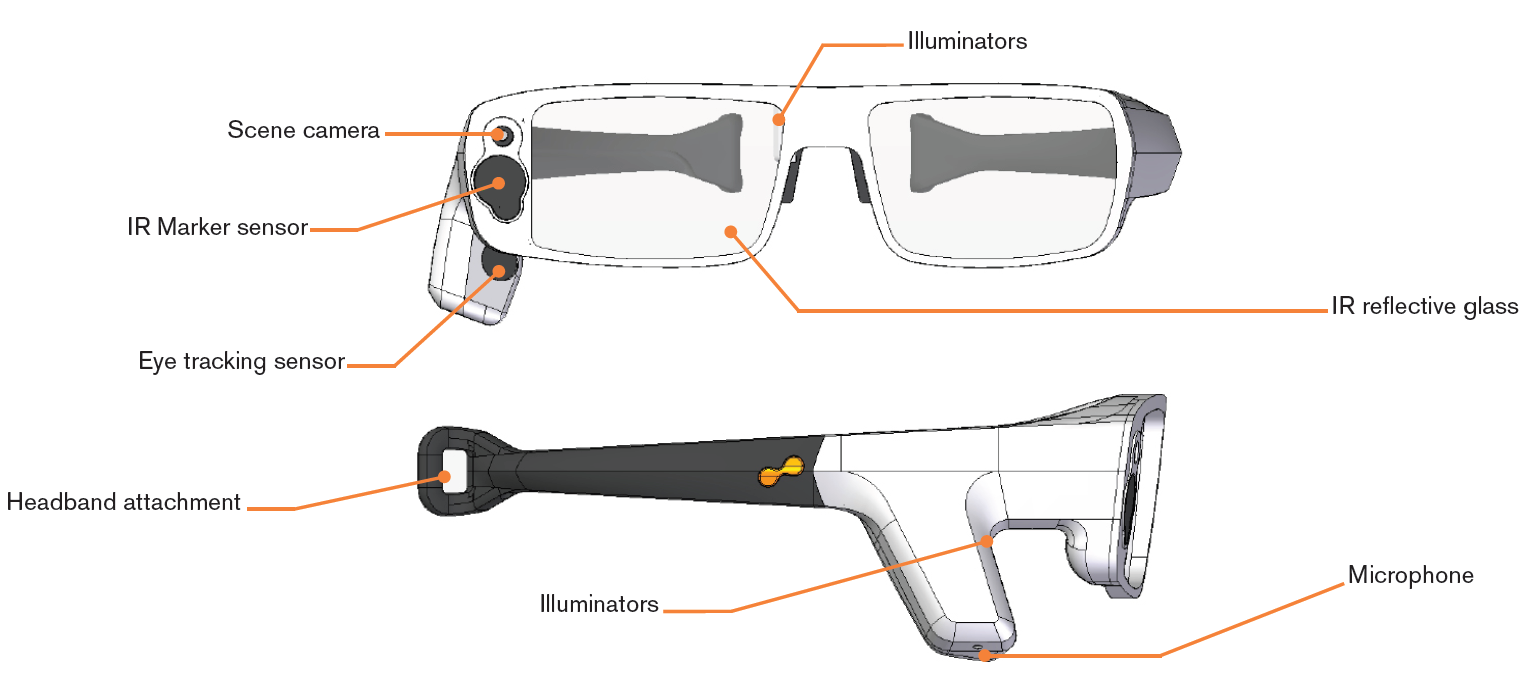
\includegraphics[scale=0.4]{TobiiGlasses}
  \caption{Tobii Glasses}
  \label{fig:TG}
\end{figure}

Le capteur infrarouge permet au système de connaitre la position de la tête de l’utilisateur dans l’espace à l’aide d’émetteurs infrarouges balisant la zone qu'il regarde (cf. figure \ref{fig:Emetteur}).

\begin{figure}[H]
  \centering
  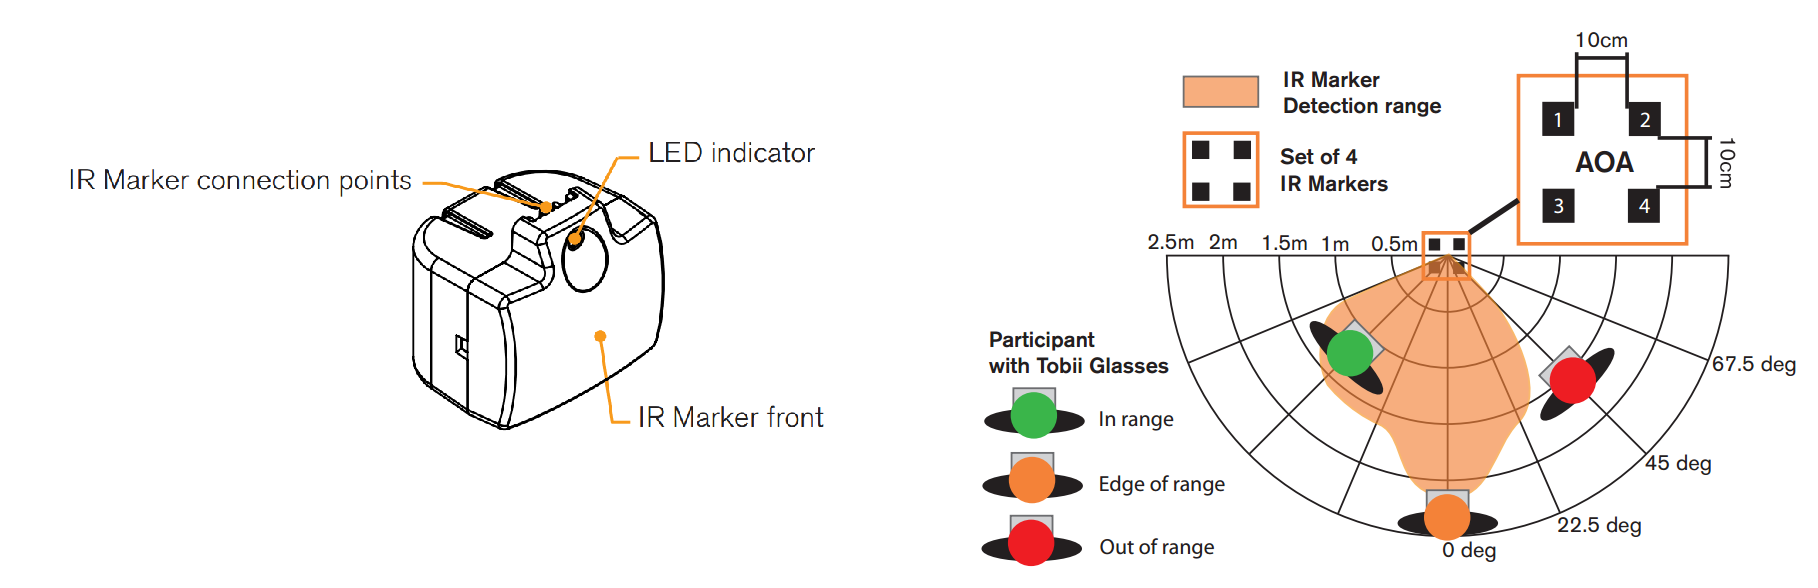
\includegraphics[scale=0.35]{BoitierTobii}
  \caption{Emetteur}
  \label{fig:Emetteur}
\end{figure}

Toutes les données sont enregistrées dans un boîtier relié aux lunettes (cf. figure \ref{fig:Boitier}). Elles peuvent ensuite être récupérées, traitées et analysées sur un ordinateur. La calibration est aussi effectuée via le boîtier.

\begin{figure}[H]
  \centering
  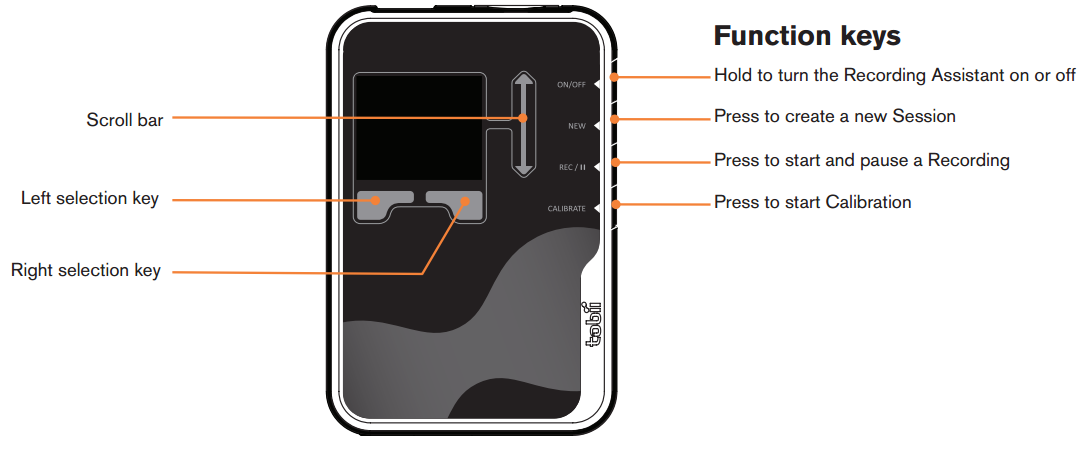
\includegraphics[scale=0.6]{BoitierTobii2}
  \caption{Boîtier}
  \label{fig:Boitier}
\end{figure}

D’un point de vue technique ces lunettes utilisent le Pupil Centre Corneal Reflection (PCCR, cf. figure \ref{fig:PCCR}). Cette méthode consiste à illuminer l’œil, créant ainsi un reflet sur la pupille et la cornée. Une caméra récupère ensuite une image de cette réflexion. Le vecteur formé par l’angle entre la cornée et le reflet lumineux sur la pupille est ensuite calculé. La direction correspond alors à la direction du regard de l’utilisateur.
Malheureusement l’algorithme de calcul n’est pas donné.

\begin{figure}[H]
  \centering
  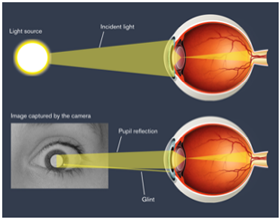
\includegraphics[scale=0.8]{PCCR}
  \caption{Pupil Centre Corneal Reflection PCCR}
  \label{fig:PCCR}
\end{figure}

Le prix n’est pas communiqué sur le site internet, mais il semblerait qu’il soit d’environ 10 000 \euro{}.

\subsubsection{PUPIL}

\begin{figure}[h]
  \centering
  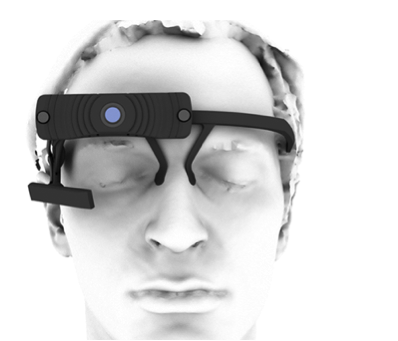
\includegraphics[scale=1]{PUPIL}
  \caption{PUPIL}
  \label{fig:PUPIL}
\end{figure}

PUPIL est un projet développé par trois étudiants du MIT. Tout comme les Tobbi Glasses il peut capter et enregistrer les mouvements effectués par l’œil de l’utilisateur.

Le principe de fonctionnement est basé sur deux caméras. La première permet d’enregistrer les mouvements de l’œil, et donc de retrouver par la suite la position de la pupille. La seconde filme ce qu’est censé voir l’utilisateur et permet de connaitre la direction du regard de l’utilisateur en utilisant les données de la première caméra.
Deux notions sont donc à distinguer : la position de la pupille et la direction du regard. La première nous aide à déduire la seconde. L’avantage de cette méthode est l’usage d'une caméra classique afin de détecter la direction du regard. Il n’est ici pas obligatoire d’employer la réflexion d’une lumière infra-rouge dans l’œil de l’utilisateur.

D’un point de vue matériel, les deux caméras utilisées sont très différentes.
Celle enregistrant le mouvement des yeux est une caméra basse résolution (640*480 à 30 fps) avec un filtre infrarouge (la  Microsoft LifeCam HD-6000 est recommandée). La caméra qui filme le monde alentour possède quant à elle une grande résolution (1920*1080, la Logitech HD 1080p Webcams est recommandée).
PUPIL peut être acheté pour la somme de 380 \euro{}.

\subsection{Systèmes sans contact}

\subsubsection{Tobii X2-30\&60}

\begin{figure}[h]
  \centering
  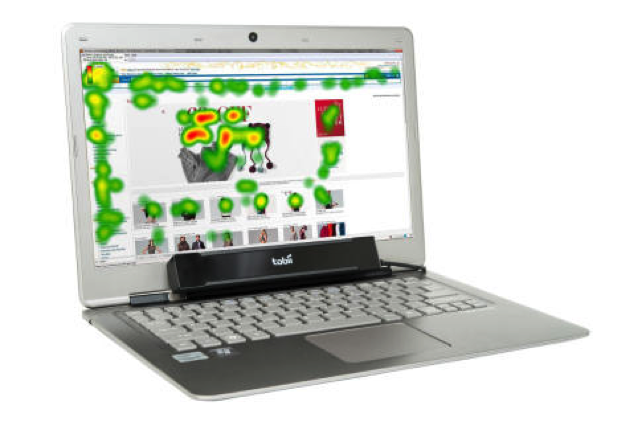
\includegraphics[scale=1]{TobiiX2}
  \caption{Tobii X2-30\&60}
  \label{fig:TobiiX2}
\end{figure}

Autre produit créé par Tobii, le X2 rentre dans les systèmes d’oculométrie sans contact. Ne mesurant que 184 mm, il se branche directement en USB. Il est très facile d’utilisation et s'adapte à de nombreux supports (ordinateurs portables, tablettes, télévisions...).
Cet outil ne permet pas de contrôler le système sur lequel il est branché mais d’enregistrer ce que l’utilisateur regarde afin d’obtenir des statistiques.
La détection de la direction du regard se fait aussi à l’aide de la réflexion causée par des LEDs infrarouges sur la cornée du sujet. Combiné avec la localisation de la pupille, le système peut en déduire la direction du regard de l’utilisateur. Encore une fois l’algorithme n’est malheureusement jamais décrit. Cependant la précision de l’appareil permet une précision d’environ 0.34° sur la direction du regard du sujet. 

\subsubsection{Eye Charm}

\begin{figure}[h]
  \centering
  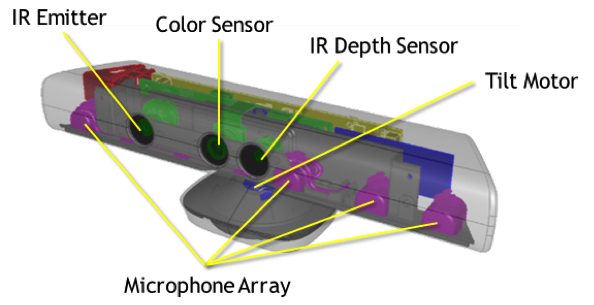
\includegraphics[scale=1]{EyeCharm}
  \caption{EyeCharm}
  \label{fig:EyeCharm}
\end{figure}

Créé par une société allemande (4tiito), EyeCharm est un adaptateur qui se clipse sur la Kinect et exploite sa caméra infrarouge pour suivre le mouvement des yeux. Un logiciel compatible avec Windows 7 \& 8 (NUIA) a été développé pour contrôler les principales fonctions d’un ordinateur grâce à ce système, comme le navigateur internet, les jeux vidéo et d’autres applications. L’utilisation d’EyeCharm ne nécessite aucun changement dans le code source des applications.
L’algorithme de suivi traite des images. La puissance de calcul nécessaire à son utilisation est ainsi assez importante (exemple : « son algorithme consomme 5 \% de la puissance d’un processeur Intel Core i5-3470 cadencé à 3,2 GHz »). Il est recommandé de détenir « un pc équipé d’un processeur AMD ou Intel multicœur et avec au moins 2 Go de mémoire vive ».
Le rôle d’EyeCharm est de projeter une lumière infrarouge sur le visage de l’utilisateur. Celle-ci est captée par la caméra de la Kinect (pour Xbox ou Windows, connectée en USB 2.0), ce qui lui permet de suivre le mouvement des yeux. Il est conseillé de se tenir à 75 cm de l’écran pour obtenir de bons résultats.

Le logiciel compte plusieurs extensions pour étendre les possibilités de contrôle par les yeux à :
\begin{itemize}[label=\textbullet,font=\color{black}]
\item plusieurs navigateurs internet (Chrome, Internet Explorer, Firefox)
\item Adobe Photoshop
\item la suite Office
\item les jeux World of Warcraft et Minecraft
\end{itemize}

Certaines fonctionnalités, comme le zoom ou le retour à la page précédente peuvent nécessiter une action supplémentaire, non réalisée par les yeux. Pour cela, il est possible d’appuyer sur une touche du clavier ou d’utiliser une commande vocale, prise en charge par la Kinect. 
Un kit de développement a été prévu pour que les utilisateurs puissent développer eux-mêmes des applications à l’aide de Qt Creator, Visual Studio, et les langages C, C++, C\# et Java.

\subsubsection{Robust Eye and Pupil Detection Method for Gaze Tracking}
\label{SystSC}

\begin{figure}[H]
  \centering
  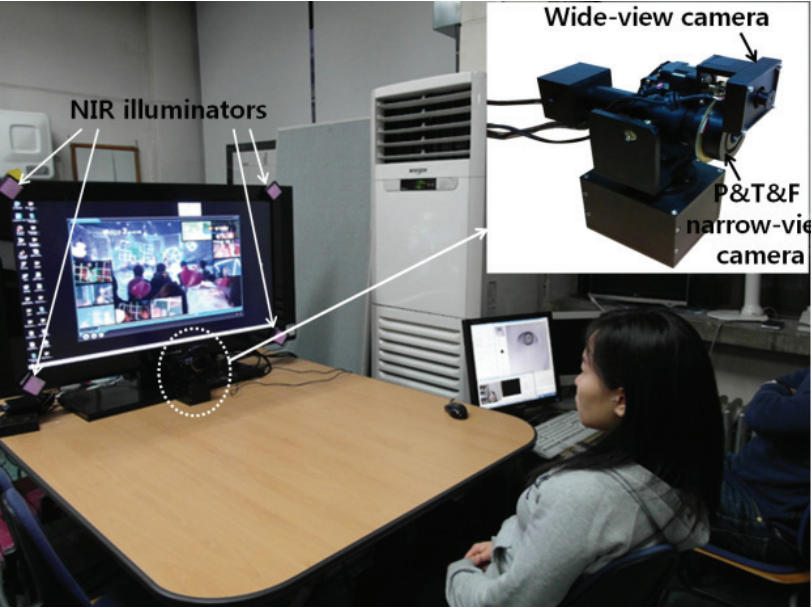
\includegraphics[scale=0.6]{Experimental}
  \caption{Robust Eye and Pupil Detection Method for Gaze Tracking}
  \label{fig:Experimental}
\end{figure}

Ce système est intéressant car il n’est pas directement embarqué sur l’utilisateur. La détection des yeux se fait à l’aide de deux caméras. Ces dernières sont motorisées et peuvent donc tourner sur elle-même ou s’orienter vers le haut ou le bas. 
Une caméra dite wide-view filme l’utilisateur dans son intégralité. Dans les faits cette caméra permet de repérer son visage, puis la position de son œil grâce à deux algorithmes de reconnaissance faciale (l’Adaboost et le CAMShift). Une fois l’œil détecté, sa position est transmise à la seconde caméra dite narrow-view (d’une résolution de 1600x1200 réduite à du 240x320 pour améliorer le temps de calcul). Elle va pouvoir zoomer sur l’œil et ainsi obtenir un gros plan, tandis que la première ne sert qu’à repérer l’usager. Une fois l’œil dans le champ de vision de la caméra, la direction de celui-ci est calculée à l’aide du centre de la pupille et des réflexions spéculaires créées sur l’œil par quatre « near-infrared illuminators », eux même placés aux quatre coins de l’écran que regarde l’utilisateur. Ici encore l’algorithme de calcul reste flou.

D’un point de vue logiciel, cette méthode emploie du C++ et la librairie OpenCV. Tous les calculs sont effectués directement sur un ordinateur classique équipé d’un processeur Intel Core 2 Quad 2.3 GHz et de 4 GB.
N’étant qu’un sujet de thèse, ce montage n’est pas en vente.

\section{La détection de pupilles}

\subsection{L’œil}

Il est important de commencer par un rappel des caractéristiques biologiques de l’œil. Le lecteur acquerra certaines notions de bases qui lui permettront de mieux appréhender les différentes problématiques de la détection de pupilles.
La figure \ref{fig:PartiesOeil} nous présente les différentes parties de l’œil.

\begin{figure}[H]
  \centering
  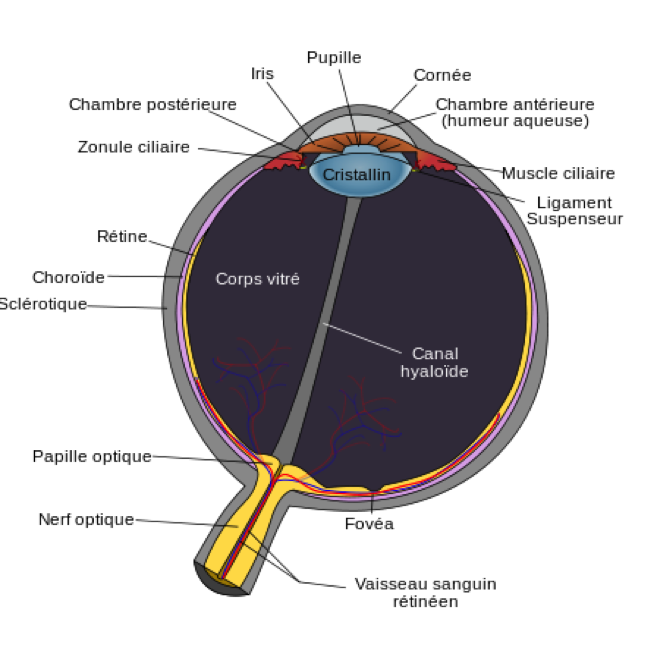
\includegraphics[scale=1]{PartiesOeil}
  \caption{Schéma anatomique de l'œil humain}
  \label{fig:PartiesOeil}
\end{figure}

Dans le cadre de la détection de pupilles, nous nous intéresserons plus particulièrement à la partie visible de l’œil. Cette partie externe est composée de 3 zones :
\begin{itemize}[label=\textbullet,font=\color{black}]
\item La partie centrale : la pupille. C’est un orifice noir permettant de laisser passer la lumière.
\item La bande colorée entourant la pupille : l’iris. Il permet de plus ou moins dilater la pupille.
\item La zone blanche qui recouvre le reste de la partie visible : la sclérotique.
\end{itemize}

La figure \ref{fig:PartiesExternesOeil} présente ces 3 parties.
\begin{figure}[h]
  \centering
  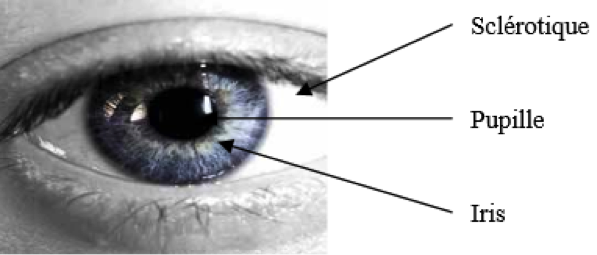
\includegraphics[scale=1]{PartiesExternesOeil}
  \caption{Les différentes parties externes de l'œil humain}
  \label{fig:PartiesExternesOeil}
\end{figure}

Nous allons maintenant nous intéresser à la capture d’une image d’un œil, à son traitement puis à la détection de la pupille.

\subsection{Caractéristiques d’une image d’un œil acquise par caméra traditionnelle}

Il existe deux types de caméras pour acquérir l'image d’un œil : la caméra traditionnelle et la caméra infrarouge. Alors que la caméra traditionnelle permet de capturer le spectre de couleurs visibles par l’œil humain, la caméra infrarouge permet de capter les ondes infrarouges de la lumière naturelle (voir figure \ref{fig:SpectreLumiere}). Cependant, la lumière naturelle ne comprend que très peu de composantes infrarouges. Ainsi, il est souvent nécessaire de soumettre l’objet d’étude (l’œil pour notre projet) à une source de lumière infrarouge supplémentaire afin d’améliorer la qualité et la luminosité de l’image acquise. La caméra infrarouge permet d’éviter la majorité des problèmes de réflexion rencontrés par une caméra traditionnelle. Nous pouvons voir figure \ref{fig:CaptureOeilTrad} et figure \ref{fig:CaptureOeilInfra} les différents types d’image.

\begin{figure}[h]
  \centering
  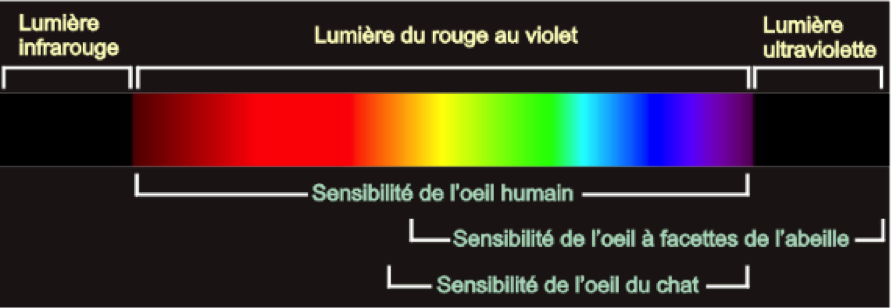
\includegraphics[scale=1]{SpectreLumiere}
  \caption{Contenu spectral de la lumière}
  \label{fig:SpectreLumiere}
\end{figure}

\begin{figure}[!h] 
\centering
\subfigure[Traditionnelle]{
  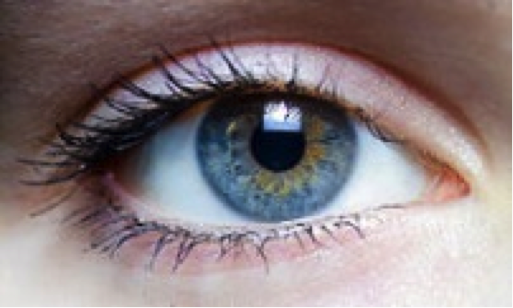
\includegraphics[scale=0.7]{CaptureOeilTrad}
  \label{fig:CaptureOeilTrad}
}
\quad 
\subfigure[Infrarouge]{
  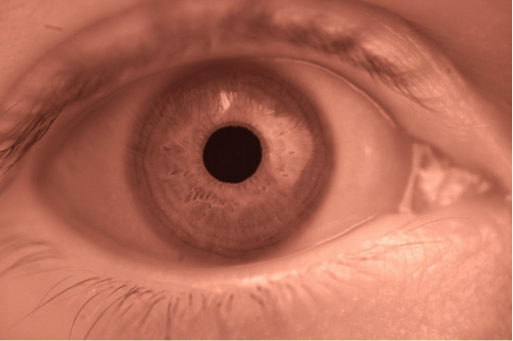
\includegraphics[scale=0.63]{CaptureOeilInfra}
  \label{fig:CaptureOeilInfra}
}
\caption{Capture d’œil à l’aide d’une caméra} 
\end{figure}

\subsection{Les différentes problématiques de la détection par caméra traditionnelle}

\subsubsection{Ombres}

La première difficulté rencontrée lors de la détection de pupilles par caméra traditionnelle est la présence de l'ombre des cils (voir figure \ref{fig:ZoneOmbre}). Cet ombrage est dû à un angle trop grand entre la source de lumière et l’axe de la pupille. Afin de réduire ce phénomène au maximum, une attention particulière doit être portée au positionnement et à l’axe de la source de lumière.

\begin{figure}[h]
  \centering
  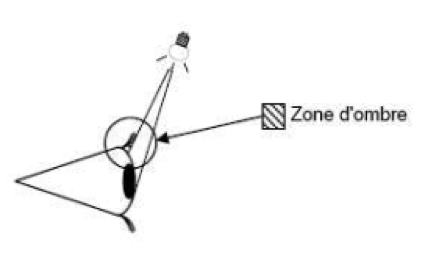
\includegraphics[scale=1]{ZoneOmbre}
  \caption{Formation d’ombre dans une image d’un œil}
  \label{fig:ZoneOmbre}
\end{figure}

\subsubsection{Reflets}

La surface de l’œil étant lisse et recouverte par la cornée, structure transparente recouvrant et protégeant l’iris (figure \ref{fig:PartiesOeil}), les reflets émanant de l’œil sont considérables. 
L’intensité des reflets sont fonction de l’intensité lumineuse dégagée par la scène. Plus la scène sera lumineuse, plus elle sera reflétée dans l’œil.

Cependant, ces reflets sont gênants pour le traitement de l’image, et plus particulièrement pour la reconnaissance de la pupille. Par exemple, la figure \ref{fig:CaptureOeilTrad} présente un œil avec un reflet recouvrant une partie de la pupille et une partie de l’iris. Ainsi, la pupille n’est plus tout à fait ronde et cela peut poser problème lors de sa détection. 

Une attention particulière devra être portée aux éclairages de la pièce afin d'éviter les réflexions lumineuses ambiantes dues aux fenêtres, lampes et néons.. Cependant, il est important de noter qu’une réduction des sources lumineuses n’est pas une solution car l’image perdrait en clarté, en qualité, et son traitement n’en serait que plus difficile. La solution réside plus dans l’harmonisation de l’éclairage afin de ne pas créer de zone de réflexion.

Plusieurs approches sont possibles pour la résolution de ce problème de réflexion : soit par l’application d’opérateurs morphologiques\footnote{La morphologie mathématique est une théorie et technique mathématique et informatique d'analyse. Son développement est inspiré des problèmes de traitement d'images, domaine qui constitue son principal champ d'application. Elle fournit en particulier des outils de filtrage, segmentation, quantification et modélisation d'images.} en dilatant puis érodant la zone atteinte par la réflexion, soit en considérant qu’un reflet possède des caractéristiques contraires à celles de la pupille. Une source lumineuse étant très claire, on peut définir des bornes de niveau de gris à partir de l’histogramme de l’image et effectuer une segmentation (opérations de traitement d’images). Le seuillage de l’image originale de la pupille et l’image arborant les zones de réflexions seront combinés afin de former une image où les trous provoqués par les sources lumineuses seront remplis.

Il faut aussi noter que le port de verres correcteurs ou de lentilles accentue le phénomène de reflets.

\subsubsection{Pupille}

Il faut noter que si l’axe de la source de lumière correspond à celui des pupilles, il en résultera un effet d’yeux rouges qui peut être gênant pour le traitement de l’image et surtout la détection des pupilles. De plus, la taille des pupilles varie en fonction de l’intensité lumineuse présente. Il faudra donc veiller à ne pas imposer une source lumineuse trop importante afin d’avoir une taille de pupille suffisamment grande pour une bonne détection.

\subsection{Détection par éclairage infrarouge}
\label{EclInfra}

La détection de la pupille par illumination de l’œil avec des éclairages infrarouges se décline en deux grandes méthodes : la méthode dite de la pupille lumineuse (brigth pupil) et celle de la pupille noire (dark pupil). Suivant la position de l’éclairage infrarouge la pupille aura des propriétés optiques différentes. Si l’illumination infrarouge est coaxiale avec l’axe optique de la caméra alors la pupille apparaitra totalement blanche (bright pupil). Au contraire si la source lumineuse est décalée (toujours par rapport à l’axe optique), alors la pupille apparaitra noire (dark pupil) et l’on pourra voir distinctement les reflets de la source lumineuse infrarouge sur la cornée du sujet.

\begin{figure}[H]
  \centering
  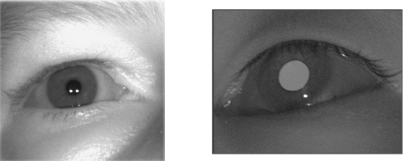
\includegraphics[scale=1]{BrightPupil}
  \caption{Effet black et bright pupil}
  \label{fig:BrightPupil}
\end{figure}

\subsection{Traitement d’images}

\subsubsection{Segmentation}

La segmentation (aussi appelée Clustering) est une étape de base du traitement d’images qui a pour but de séparer différentes zones homogènes d’une image en groupes (clusters) dont les membres ont en commun diverses propriétés (intensité, couleur, texture...). En d’autres mots, cette opération rassemble des pixels entre eux suivant des critères prédéfinis. Les pixels sont ainsi regroupés en régions, qui constituent un pavage ou une partition de l'image. Il peut s'agir par exemple de séparer les objets du fond. On peut regrouper les différentes méthodes de segmentation en deux catégories : la segmentation non supervisée, qui vise à séparer automatiquement l’image en différents clusters naturels (sans aucune connaissance préalable des classes) ; et la segmentation supervisée, qui s’opère à partir de la connaissance de chacune des classes définies par une approche probabiliste. Concernant les méthodes de segmentation non supervisée, nous nous intéresserons à deux méthodes : le Fuzzy C-means et le k-means. 

\subsubsection*{Description des algorithmes}
Fuzzy C-Means (FCM) est un algorithme de classification non supervisée floue. Il introduit la notion d’ensemble flou dans la définition des classes : chaque point (pixel) dans l’ensemble des données appartient à chaque cluster avec un certain degré d’appartenance, et tous les clusters sont caractérisés par leur centre de gravité. Ainsi, il permet d’obtenir une partition floue de l’image en donnant à chaque pixel un degré d’appartenance compris entre 0 et 1 à un cluster donné. Le cluster auquel est associé un pixel est celui dont le degré d’appartenance est le plus élevé.

Les principales étapes de l’algorithme Fuzzy C-means sont :
\begin{enumerate}
\item La fixation arbitraire d’une matrice des classes.
\item Le calcul des centroïdes des classes.
\item Le réajustement de la matrice d’appartenance suivant la position des centroïdes.
\item Calcul du critère de minimisation et retour à l’étape 2 s’il y a non convergence de critère.
\end{enumerate}
\paragraph{}
L’algorithme k-means est l’algorithme de Clustering le plus connu et le plus utilisé (simple à mettre en œuvre). Il permet de partitionner les pixels d’une image en K clusters. L’algorithme k-means ne crée qu’un seul niveau de clusters. Il renvoie une partition des données, dans laquelle les objets à l’intérieur de chaque cluster sont aussi proches que possible les uns des autres et aussi loin que possible des objets des autres clusters. Chaque cluster de la partition est défini par ses objets et son centroïde. Le k-means est un algorithme itératif qui minimise la somme des distances entre chaque objet et le centroïde de son cluster. La position initiale des centroïdes conditionne le résultat final, de sorte qu'ils doivent être initialement placés le plus loin possible les uns des autres de façon à optimiser l’algorithme. K-means réitère ses opérations jusqu’à ce que la somme ne puisse plus diminuer. Le résultat est un ensemble de clusters compacts et clairement séparés, à condition d’avoir choisi la bonne valeur K du nombre de clusters. Les principales étapes de l’algorithme k-means sont :
\begin{enumerate}
\item Choix aléatoire de la position initiale des K clusters.
\item (Ré-)Affecter les objets à un cluster suivant un critère de minimisation des distances (généralement selon une mesure de distance euclidienne).
\item Une fois tous les objets placés, recalculer les K centroïdes.
\item Réitérer les étapes 2 et 3 jusqu’à ce que plus aucune réaffectation ne soit faite.
\end{enumerate}
\paragraph{}
Statistics Toolbox implémentée sous MatLab 7 contient la fonction kmeans.m, facile à prendre en main et bien documentée et Fuzzy Logic Toolbox contient fcm.m.

\subsubsection*{Comparaison}
Il apparait que ces deux algorithmes sont assez efficaces pour des images couleurs et permettent une bonne segmentation. Cependant, lors de la présence de défauts (reflets, ombres...), la segmentation parait correcte (elle ne permet pas une bonne détection des caractères par Optical Character Recognition OCR, ce qui ne nous intéresse pas). Enfin, il apparait que ces algorithmes ne sont pas adaptés à des images contenant un grand nombre d’objets (au niveau du temps de calcul). La méthode FCM semble plus efficace pour la haute résolution, et au contraire, k-means convient plus aux images à faible résolution.

\subsubsection{Traitement de l’image pour la détection de pupilles}

La détection des pupilles est composée de plusieurs étapes et peut être codée à l’aide de plusieurs méthodes différentes en fonction de la complexité choisie. Certaines méthodes sont plus complexes et meilleures mais plus longues à réaliser (au niveau du temps de calcul). Pour notre projet, nous avons besoin de faire du traitement d’images en temps réel donc nous devrons faire attention à la complexité de notre algorithme. Les différentes étapes de la détection de la pupille sont : 
\begin{enumerate}
\item Filtrage du bruit (filtre médian...).
\item Prétraitement (égalisation histogramme + seuillage bas pour supprimer le reflet).
\item Extraction de contour (filtre variance, ...).
\item Recherche des cercles/ellipses (Hough).
\item Discrimination du cercle de la pupille (couleur, position, surface, ...).
\end{enumerate}
\paragraph{}
Une première méthode de détection de la pupille, développée par Jérôme Schmaltz de l’Ecole de Technologie Supérieure de Montréal, repose sur le principe décrit figure \ref{fig:TraitementImage}.
\begin{figure}[h]
  \centering
  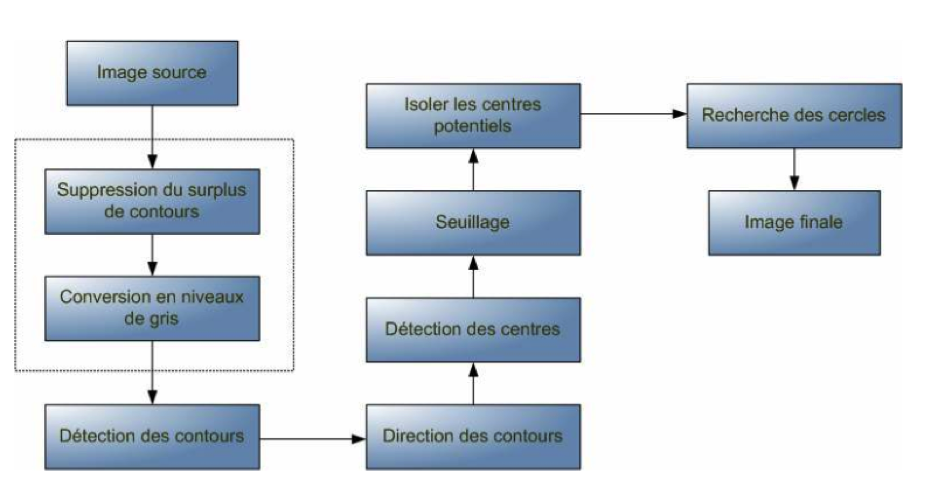
\includegraphics[scale=1]{TraitementImage}
  \caption{Différentes étapes de traitement de l’image afin de détecter une pupille dans une image.}
  \label{fig:TraitementImage}
\end{figure}

\subsubsection*{Suppression de surplus de contours, atténuation du bruit}
\label{Filtre}

Tout d’abord, il est nécessaire de réduire le bruit occasionné par la caméra, le bruit engendré par le transfert des données et leur compression. Différents filtres peuvent être utilisés, même si leur application altérera les contours de l’image. 

\subsubsection*{Filtre Moyenneur}

Ce filtre lisseur part du principe que la valeur d'un pixel est relativement similaire à son voisinage. Il fait donc en sorte que chaque pixel soit remplacé par la moyenne pondérée de ses voisins. Si on applique un filtre moyenneur de taille $\lambda$=3, cela signifie qu'on additionne la valeur de tous les pixels du voisinage du pixel traité. On obtient ainsi la matrice de convolution suivante :
$$h = \frac{1}{9}
\begin{bmatrix}
	1 & 1 & 1 \\
	1 & 1 & 1 \\
	1 & 1 & 1 \\
\end{bmatrix}  $$

\paragraph{}
h s’appelle le masque de convolution. La somme des coefficients du masque valant 1, le lissage préservera toute zone de l’image où le niveau de gris est constant. Ce filtre peut engendrer des phénomènes de fausses couleurs, contrairement au filtre médian car son efficacité est moindre lorsque les objets présents dans l'image sont de faible dimension par rapport aux dégradations. Ce filtre est isotrope. 

Une amélioration du filtre moyenneur consiste à jouer sur les valeurs des coefficients du masque :
$$h = \frac{1}{10}
\begin{bmatrix}
	1 & 1 & 1 \\
	1 & 2 & 1 \\
	1 & 1 & 1 \\
\end{bmatrix}  $$

\subsubsection*{Coupe Médiane}

Une coupe médiane permet d’atténuer le bruit d’une image. Le principe est de prendre dans le voisinage la valeur la moins extrême. Pour cela, on crée une liste des valeurs du voisinage, puis on trie cette liste et on prend la valeur qui se trouve au milieu de la liste. Cette valeur "médiane" est la plus éloignée des deux extrêmes.

\subsubsection*{Diffusion}

Le principe est d’atténuer les différences d'intensité entre le pixel central et ses voisins. Pour chaque voisin, on calcule la différence d'intensité avec le pixel central. Plus la différence est faible, plus elle est propagée vers le pixel central. Cela permet d'uniformiser les zones d'intensité proche et de conserver les forts contrastes (et donc les contours).

\subsubsection*{Filtre Gaussien}
\label{FiltreGaussien}

Le filtre Gaussien est un filtre isotrope spécial avec des propriétés mathématiques bien précises. $\sigma$ caractérise l'écart type soit la largeur du filtre : autrement dit la largeur du filtre en partant du point central est égale à 3$\sigma$ arrondi à l'entier supérieur. En deux dimensions, le filtre de Gauss est le produit de deux fonctions gaussiennes, une pour chaque direction :

$$g(x,y) = \frac{1}{2\pi\sigma^2}\cdot \mathrm{e}^{-\frac{x^2+y^2}{2\sigma^2}}$$

L’effet de ce filtre sur l’image est assez similaire au filtre moyenneur, mais la moyenne est pondérée : les pixels près du centre ont un poids plus important que les autres. En général, un filtre Gaussien avec $\sigma$<1 est utilisé pour réduire le bruit, et si $\sigma$>1 c’est dans le but de flouter volontairement l'image. Il faut noter que plus $\sigma$ est grand, plus la cloche Gaussienne est large, et plus le flou appliqué à l’image sera marqué.

\subsubsection{Conversion en niveau de gris}

La seconde étape du prétraitement consiste à convertir l’image RGB en niveau de gris. Cette conversion est nécessaire puisque les différents algorithmes se basent sur des images en niveau de gris. On pourrait d’abord penser que le niveau de gris se calcule comme la somme des 3 pixels divisée par 3 : $Gris = \frac{R + G + B}{3}$

Cependant, d’après les recommandations de la commission internationale de l’éclairage, il devrait plutôt être de la forme : $Gris = 0.299R + 0.587G + 0.114B$
Nous pouvons voir figure \ref{fig:Conversion} le rendu de cette conversion.

\begin{figure}[h]
  \centering
  
\includegraphics[scale=1]{Conversion}
  \caption{Conversion en niveau de gris}
  \label{fig:Conversion}
\end{figure}

\subsubsection{Détection des contours}

\subsubsection*{Filtre de Canny}

Il existe différentes méthodes de détection des contours. Des filtres peuvent être utilisés (voir paragraphe \ref{Filtre}). Le choix du filtre doit prendre en compte qu’une réduction trop importante du bruit masque certains contours, mais qu’une réduction trop faible peut laisser apparaitre trop de contours non significatifs. Nous nous intéresserons ici au meilleur filtre pour la détection de contours : le filtre de Canny. Il est considéré comme tel car il offre un très bon compromis entre la réduction du bruit et la localisation des contours. Les différentes étapes du filtre de Canny sont :
\begin{itemize}[label=\textbullet,font=\color{black}]
\item Réduction du bruit grâce à la convolution d’un filtre passe-bas Gaussien, ce qui permet de tamiser les contours.
\item Eclaircissement des contours grâce à l’utilisation des valeurs des amplitudes des gradients ainsi que leurs directions. Pour cela, nous utilisons les formules \eqref{eq:g} et \eqref{eq:theta}.
\end{itemize}

\begin{equation}
g = \sqrt{g_x^2 + g_y^2}
\label{eq:g}
\end{equation}
\begin{equation}
\theta = \arctan{\frac{g_y}{g_x}}
\label{eq:theta}
\end{equation}

Nous pouvons voir que l’amplitude est proportionnelle à $g_x$ et $g_y$, ce qui montre qu’elle mesure la force d’un contour indépendamment de sa direction. 
\begin{itemize}[label=\textbullet,font=\color{black}]
\item Suppression des non maximaux, cela permet de réduire la largeur des arrêtes détectées à un pixel. La figure \ref{fig:Algo} décrit un algorithme permettant de supprimer ces non maximaux.
\begin{figure}[h]
  \centering
  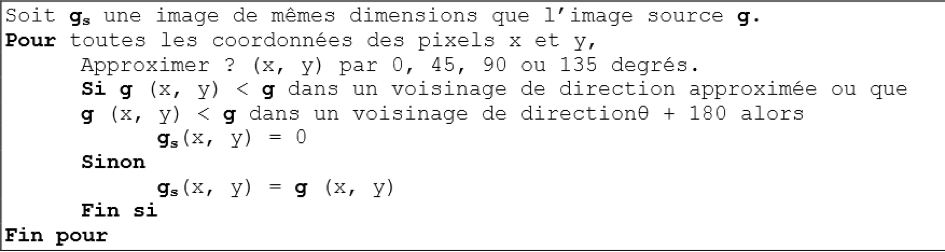
\includegraphics[scale=0.9]{Algo}
  \caption{Algorithme permettant de supprimer des non maximaux}
  \label{fig:Algo}
\end{figure}
\item Localisation : elle repose sur l’identification des contours significatifs à partir des amplitudes des gradients précédemment calculés. 
\end{itemize}

La méthode triviale consiste à appliquer un seuillage aux gradients calculés. Cependant, l’application d’un seuil trop faible implique la prise en compte de tous les contours, y compris les contours non significatifs (prise en compte des gradients maximaux engendrés par le bruit). De plus, l’application d’un seuil trop élevé engendre une fragmentation des chaines de pixels qui forment des contours significatifs de l’image. Ainsi, le seuil par hystérésis offre une bonne solution à ce problème. 

La figure \ref{fig:DetectionContours} illustre l’idée de détection des contours grâce au filtre de Canny.
\begin{figure}[H]
  \centering
  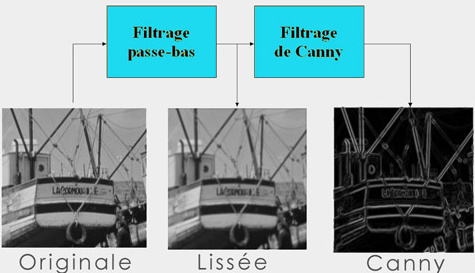
\includegraphics[scale=1]{DetectionContours}
  \caption{Détection des contours grâce au filtre de Canny}
  \label{fig:DetectionContours}
\end{figure}

\subsubsection*{Filtre de Sobel}

L'opérateur calcule le gradient de l'intensité de chaque pixel. Celui-ci indique la direction de la plus forte variation (du clair au sombre), ainsi que le taux de changement dans cette direction. On connaît alors les points de changement soudain de luminosité, correspondant probablement à des bords, ainsi que l'orientation de ces bords.
L'opérateur utilise des matrices de convolution. La matrice (généralement de taille 3×3) subit une convolution avec l'image pour calculer des approximations des dérivées horizontale et verticale. Soit $A$ l'image source, $G_x$ et $G_y$ deux images qui en chaque point contiennent des approximations respectivement de la dérivée horizontale et verticale de chaque point. Ces images sont calculées comme suit:

$$G_x = 
\begin{bmatrix}
	1 & 0 & -1 \\
	2 & 0 & -2 \\
	1 & 0 & -1 \\
\end{bmatrix}
* A \text{ et } G_y =
\begin{bmatrix}
	1 & 2 & 1 \\
	0 & 0 & 0 \\
	-1 & -2 & -1 \\
\end{bmatrix}
* A
$$

En chaque point, les approximations des gradients horizontaux et verticaux peuvent être combinées comme suit pour obtenir une approximation de la norme du gradient : $G = \sqrt{G_x^2 + G_y^2}$

On peut également calculer la direction du gradient comme suit : $\Theta = atan2(G_y, G_x)$, et créer une matrice des directions.

\begin{figure}[h]
  \centering
  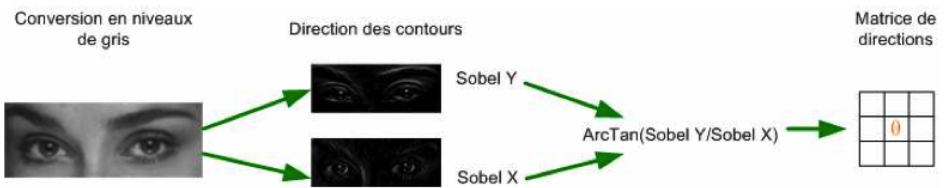
\includegraphics[scale=1]{FiltreSobel}
  \caption{Déterminer les directions des gradients à partir de l’application du filtre de Sobel}
  \label{fig:FiltreSobel}
\end{figure}

Enfin, d’autres filtres tels que le filtre de Kirsch, le filtre MDIF, le filtre de Prewitt ou encore celui de Roberts, permettent aussi la détection de contours, mais nous ne les détaillerons pas ici.

\subsubsection{Détection des centres}

Le principe de la détection des centres se base sur les deux étapes précédentes. Pour chaque point des contours de l’image de Canny, on trace une droite en fonction de la direction calculée par le biais de l’application des filtres de Sobel. Ainsi, par l’application de la formule de la droite $y = m \cdot x + b$, on trace une droite dans l’accumulateur en fonction des points de contours de l’image de Canny tels qu’exposés dans la figure \ref{fig:Contour}.

\begin{figure}[h]
  \centering
  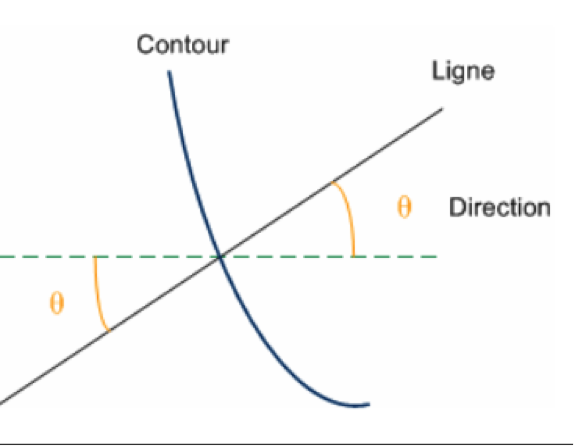
\includegraphics[scale=1]{Contour}
  \caption{Traçage d’une droite en fonction d’un contour}
  \label{fig:Contour}
\end{figure}

Tracer une droite dans un accumulateur revient à incrémenter chaque cellule d’une matrice aux endroits où elle passe (voir figure \ref{fig:Accumulateur}).

\begin{figure}[h]
  \centering
  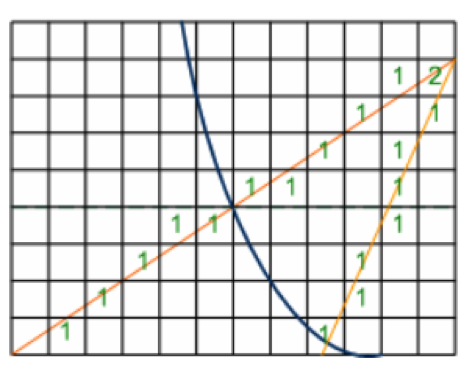
\includegraphics[scale=1]{Accumulateur}
  \caption{Traçage d’une droite dans l’accumulateur}
  \label{fig:Accumulateur}
\end{figure}

Ainsi, suivant ce principe, les valeurs maximales de la matrice indiqueront les différents centres potentiels. La figure \ref{fig:MethodeCanny} synthétise la méthode énoncée. 

\begin{figure}[h]
  \centering
  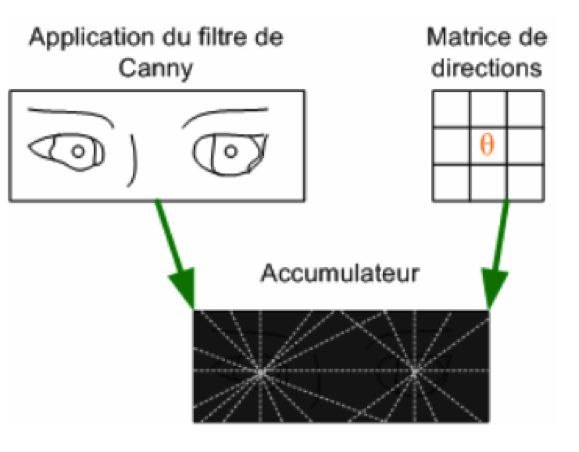
\includegraphics[scale=0.9]{MethodeCanny}
  \caption{Traçage des lignes dans l’accumulateur en fonction de l’image de Canny et de la matrice de directions}
  \label{fig:MethodeCanny}
\end{figure}

\subsubsection{Seuillage}

Le seuillage permet de désencombrer la matrice accumulateur des informations superflues. Nous recherchons les centres potentiels et ainsi nous n’avons pas besoin de toutes les valeurs de l’accumulateur. En effet, il suffit d’appliquer un seuil et de garder les pixels ayant une valeur supérieure à celui-ci (les autres pixels seront mis à zéro) car ils représenteront les différents centres potentiels. 

Pour ce faire, nous pouvons par exemple utiliser un seuil du type :

$\text{valeur pixel actuel} > 0.5 \cdot max(\text{valeur pixel image})$, qui permet de garder les pixels ayant au moins la moitié de la valeur maximale d’une cellule de l’accumulateur.

Nous pouvons voir figure \ref{fig:SeuilAccumu} le résultat du seuillage.

\begin{figure}[h]
  \centering
  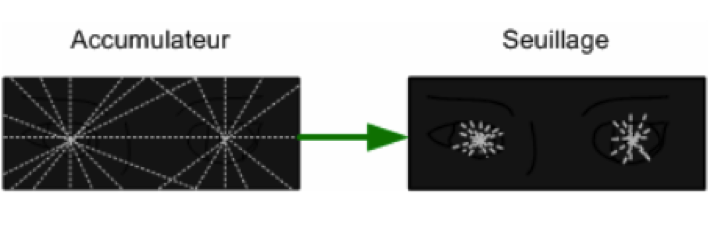
\includegraphics[scale=1]{SeuilAccumu}
  \caption{Application d’un seuil dans l’accumulateur}
  \label{fig:SeuilAccumu}
\end{figure}

\subsubsection{Isoler les centres potentiels}

L’application d’une convolution d’un chapeau mexicain (voir formule \eqref{eq:RepLaplacienGaussien} et figure \ref{fig:LaplacienGaussien}) sur l’accumulateur permet d’isoler les points les plus au centre. Un chapeau mexicain est la combinaison d’un filtre Gaussien (voir paragraphe \ref{FiltreGaussien}) avec un filtre Laplacien.

\begin{equation}
\nabla^2G_\sigma(r) = \frac{-1}{2\pi\sigma^4}(2-\frac{r^2}{\sigma^2}) \mathrm{e}^{\frac{-r^2}{2\sigma^2}}
\label{eq:RepLaplacienGaussien}
\end{equation}

\begin{figure}[H]
  \centering
  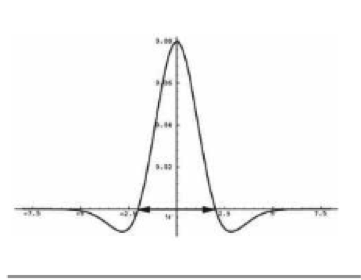
\includegraphics[scale=1]{LaplacienGaussien}
  \caption{Représentation graphique d’un Laplacien de Gaussien}
  \label{fig:LaplacienGaussien}
\end{figure}

Ainsi, l’application d’un chapeau mexicain sur l’accumulateur permet de conserver les points les plus à même d’être les centres de cercles potentiels en décrémentant les valeurs des cellules entourant les centres. La figure \ref{fig:ChapeauMexicain} présente le résultat de cet isolement des centres.

\begin{figure}[H]
  \centering
  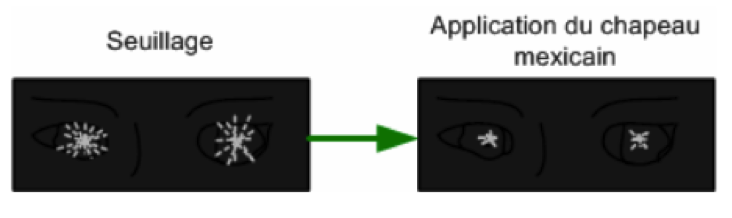
\includegraphics[scale=1]{ChapeauMexicain}
  \caption{Application d’un chapeau mexicain dans l’accumulateur}
  \label{fig:ChapeauMexicain}
\end{figure}

\subsubsection{Recherche des cercles}

La recherche des cercles s’appuie sur la création d’accumulateurs et la transformée de Hough. En effet, pour un cercle de rayon inconnu, nous utilisons des accumulateurs en 3 dimensions : les deux premières servent à ranger les coordonnées x et y du centre du cercle et la troisième permet de ranger le rayon r du cercle. 

\begin{enumerate}
\item On initialise les accumulateurs.
\item A partir de l’image des contours de Canny, on trace littéralement des cercles dans un des accumulateurs en faisant coïncider les centres des cercles avec les coordonnées du pixel de contour pour un rayon donné. La méthode de Bresenham pourra être employée afin de tracer plus efficacement les cercles dans l’accumulateur de Hough.
\item Comme on peut le voir figure \ref{fig:CerclesContours}, plusieurs cercles sont tracés (dans un accumulateur de rayon r) en suivant les contours de l’image de Canny. Nous pouvons voir que les cellules contenant les valeurs maximales coïncident avec des centres de cercles potentiels.

\begin{figure}[H]
  \centering
  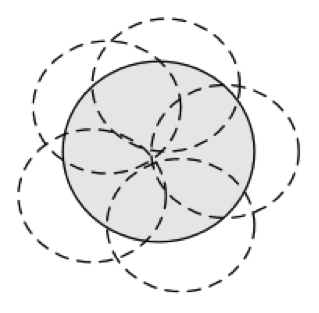
\includegraphics[scale=1]{CerclesContours}
  \caption{Traçage des cercles avec l’image des contours}
  \label{fig:CerclesContours}
\end{figure}

\item Ensuite, on peut diviser la zone d’intérêt de l’image en deux parties : partie droite et partie gauche du visage. Pour chacune de ces parties, on applique un seuil aux accumulateurs d’Hough permettant de conserver les centres, les coordonnées et rayons de cercles potentiels et on vérifie qu’ils font bien partie de l’accumulateur des cercles potentiels de l’étape de l’isolement des centres potentiels.
\item Pour finir, une moyenne des positions et des rayons des cercles restants permet une identification des cercles entourant l’iris et la pupille (à gauche et à droite). Il ne reste plus qu’à conserver le cercle ayant le rayon le plus petit, correspondant à la pupille.
\end{enumerate}

La figure \ref{fig:OpPupilles} résume cette démarche.

\begin{figure}[H]
  \centering
  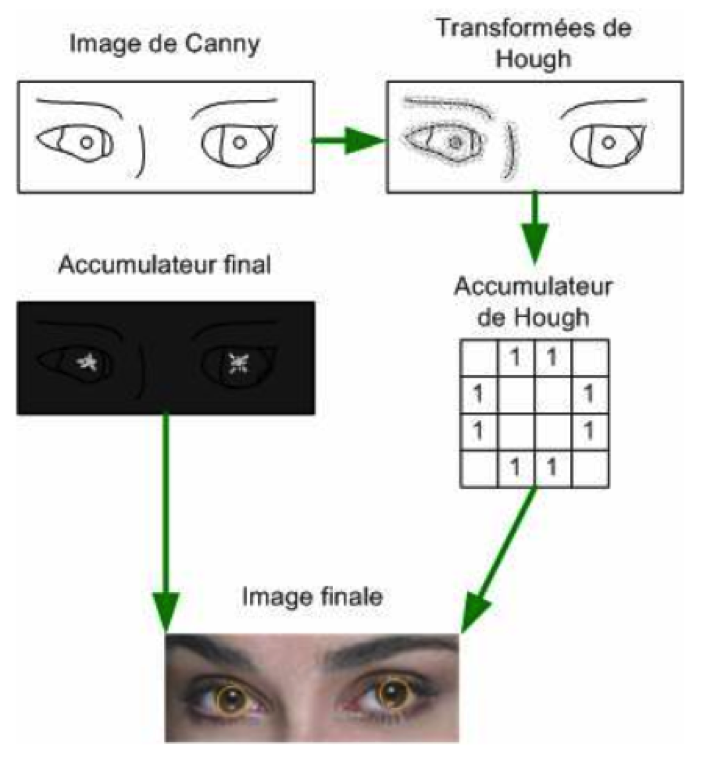
\includegraphics[scale=0.7]{OpPupilles}
  \caption{Les différentes opérations permettant de localiser les pupilles}
  \label{fig:OpPupilles}
\end{figure}

\section{Méthode de détection de la direction du regard}
\label{MethodeDirectionRegard}

La direction du regard d’une personne peut être obtenue à l’aide de deux paramètres : 
L’orientation du visage et l’orientation oculaire. La détection du visage permet de connaitre l’orientation globale de l’utilisateur et de vérifier que ses deux yeux sont bien en face de la caméra. Suivant l’orientation de la tête de l’utilisateur, une approximation de la direction du regard peut aussi être réalisée.
La détection effectuée à l’aide de l’orientation oculaire approche la direction du regard à l’aide de propriétés géométriques et physiques de l’iris et de la pupille. Le problème principal réside dans le fait que cette étude est une étude locale, c’est-à-dire que la caméra qui filme l’œil de l’utilisateur doit avoir un fort niveau de zoom, obligeant le sujet à rester immobile afin de ne pas sortir du champ de la caméra.

Les reflets détectés dans l’œil du sujet par la détection de pupille avec infrarouge (voir paragraphe \ref{EclInfra}) vont permettre de déterminer la direction du regard de l’utilisateur. En supposant la tête de l’utilisateur immobile, et en prenant comme référence le reflet formé par la lumière infrarouge sur la cornée, on peut déterminer la direction du regard en se servant du vecteur crée entre le reflet et le centre de la pupille (ou l’iris) (voir figure ci-dessous). Cependant cette méthode demande certains prérequis et notamment une calibration et ce avec chaque nouvel utilisateur. Pour effectuer cette calibration, il est demandé au sujet de fixer quatre points (minimum), situés sur l’écran, afin d’obtenir des valeurs étalons (souvent les coins de l’écran), qui permettront de déduire la direction du regard par la suite.

\begin{figure}[H]
  \centering
  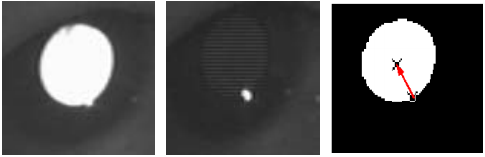
\includegraphics[scale=1]{GazeDetection}
  \caption{Tracé du vecteur entre la réflexion infrarouge dans la cornée et la pupille}
  \label{fig:GazeDetection}
\end{figure}

Cette méthode présente tout de même deux défauts majeurs : l’impossibilité pour l’utilisateur de bouger la tête ou le corps, sous risque de devoir recommencer la calibration, et l’obligation de re-calibrer le système à chaque changement d’utilisateur.

\section{Solutions techniques et méthodes choisies} 

Suite à l’état de l’art, la méthode d’eye tracking sans contact a été retenue (pas de système embarqué). Elle est similaire à celle de la partie \ref{SystSC} et semble plus facilement réalisable qu'un système utilisant des lunettes avec caméras embarquées. Ainsi, dans un premier temps, cette technique sera développée afin d’obtenir un système qui fonctionne correctement. Puis, le système pourra être perfectionné et, s’il reste du temps sur les délais fixés, la méthode utilisant des lunettes sera approfondie. 

Pour l'approche sans contact, deux caméras seront utilisées. La première, la caméra dite "grand angle", permettra de filmer la scène dans son ensemble et de localiser le visage ainsi que certains de ses éléments morphologiques tels que les oreilles et la bouche. Elle transmettra ensuite les coordonnées spatiales du visage à la seconde caméra "petit angle". Cette dernière zoomera sur le visage (grâce aux coordonnées fournies) et effectuera un tracking des pupilles.  

La détection de la pupille s’effectuera à l’aide de la méthode de la bright et de la black pupille. Les différentes étapes vues dans l’état de l’art seront respectées et des tests seront menés afin de déterminer la meilleure solution pour réaliser chaque étape.
 
Le calcul de la direction du regard s’appuiera sur la méthode vue dans la partie \ref{MethodeDirectionRegard}. Des LEDs infrarouges, placées devant l’utilisateur, illumineront sa cornée, créant une réflexion spéculaire exploitable pour estimer la direction du regard. La caméra "petit angle" devra ainsi être munie d’un filtre infrarouge. Ce filtre pourra être réalisé à l’aide d’une pellicule photo placée devant l’objectif de la caméra.  

%----------------------------------------------------------------------------------------
%	PART II 
%----------------------------------------------------------------------------------------
\part{Dossier fonctionnel}
\chapter{Dossier fonctionnel}
\section{Ingénierie des exigences}
\subsection{Approche Top-Down}
\label{sec:top-down}

Pour notre approche Top-Down, nous sommes revenus à la demande initiale du projet : remplacer la souris d'un ordinateur par le mouvement oculaire de l'utilisateur. La fonction principale du système est donc apparue clairement : permettre à l'utilisateur d'interagir avec une interface via ses yeux. 

\begin{figure}[h]
  \centering
  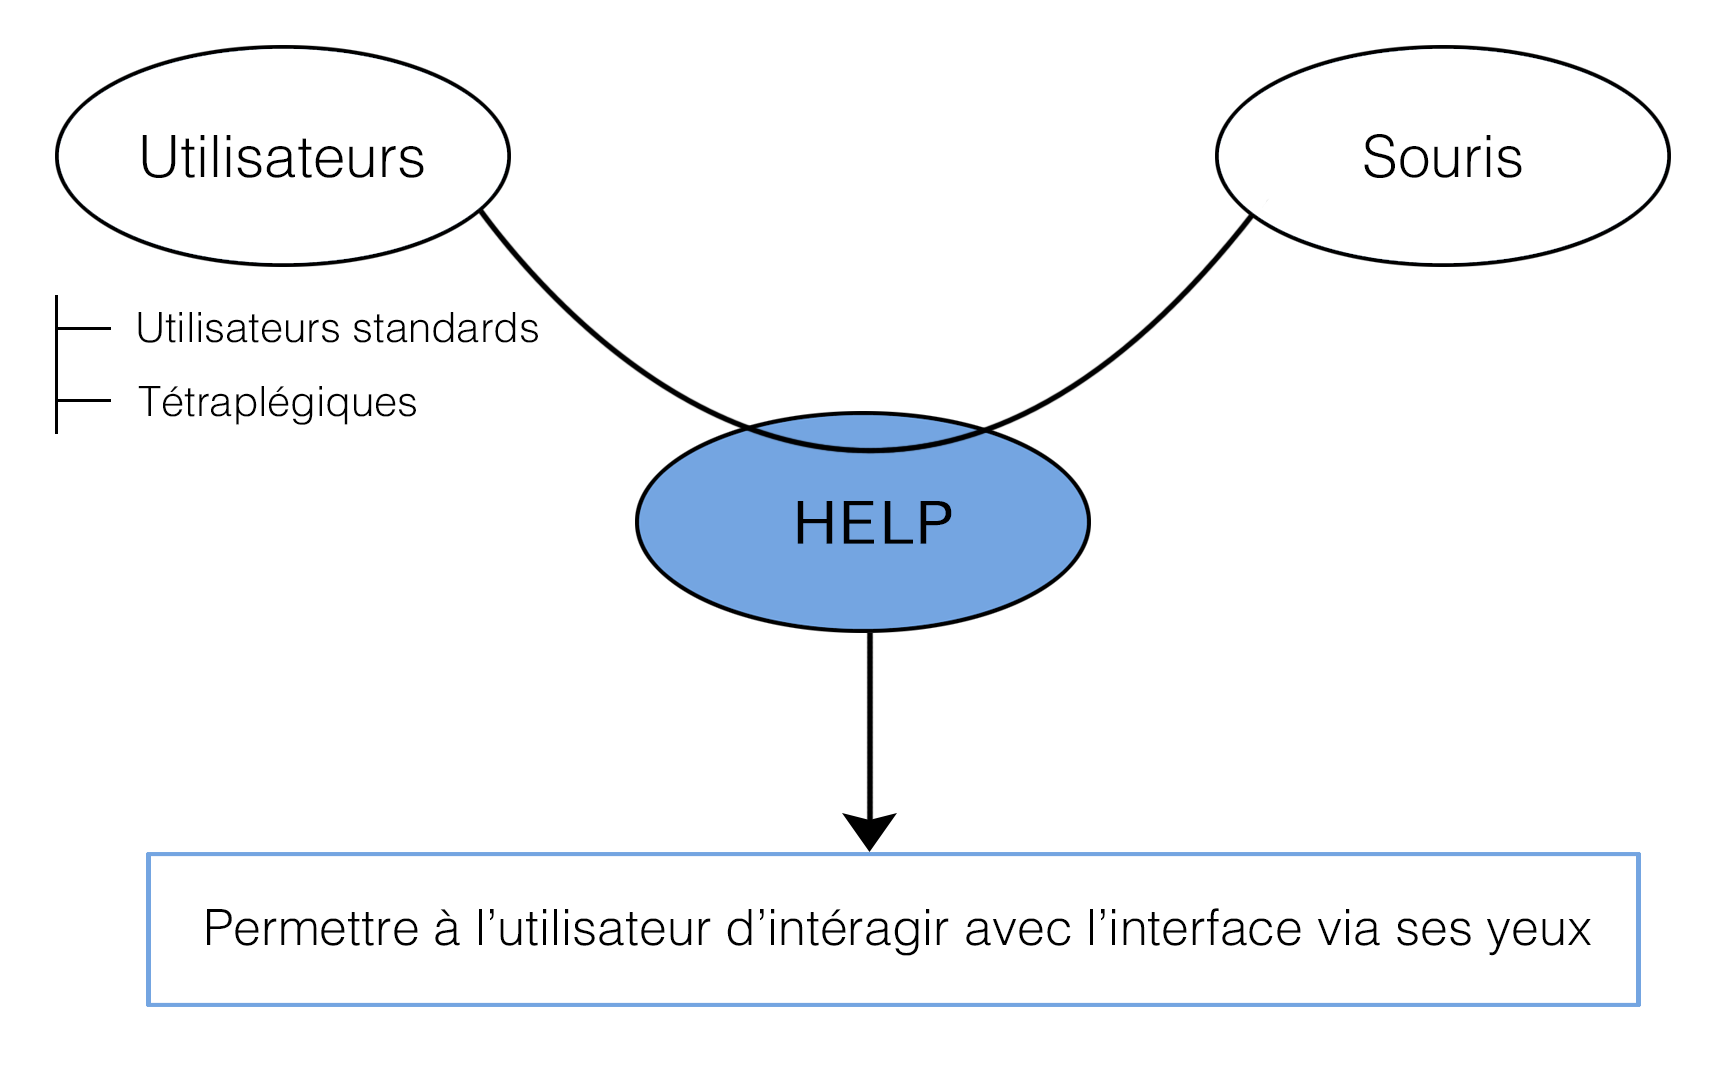
\includegraphics[scale=1]{BeteACornes}
  \caption{Bête à cornes}
  \label{fig:bac}
\end{figure}

\begin{figure}[H]
  \centering
  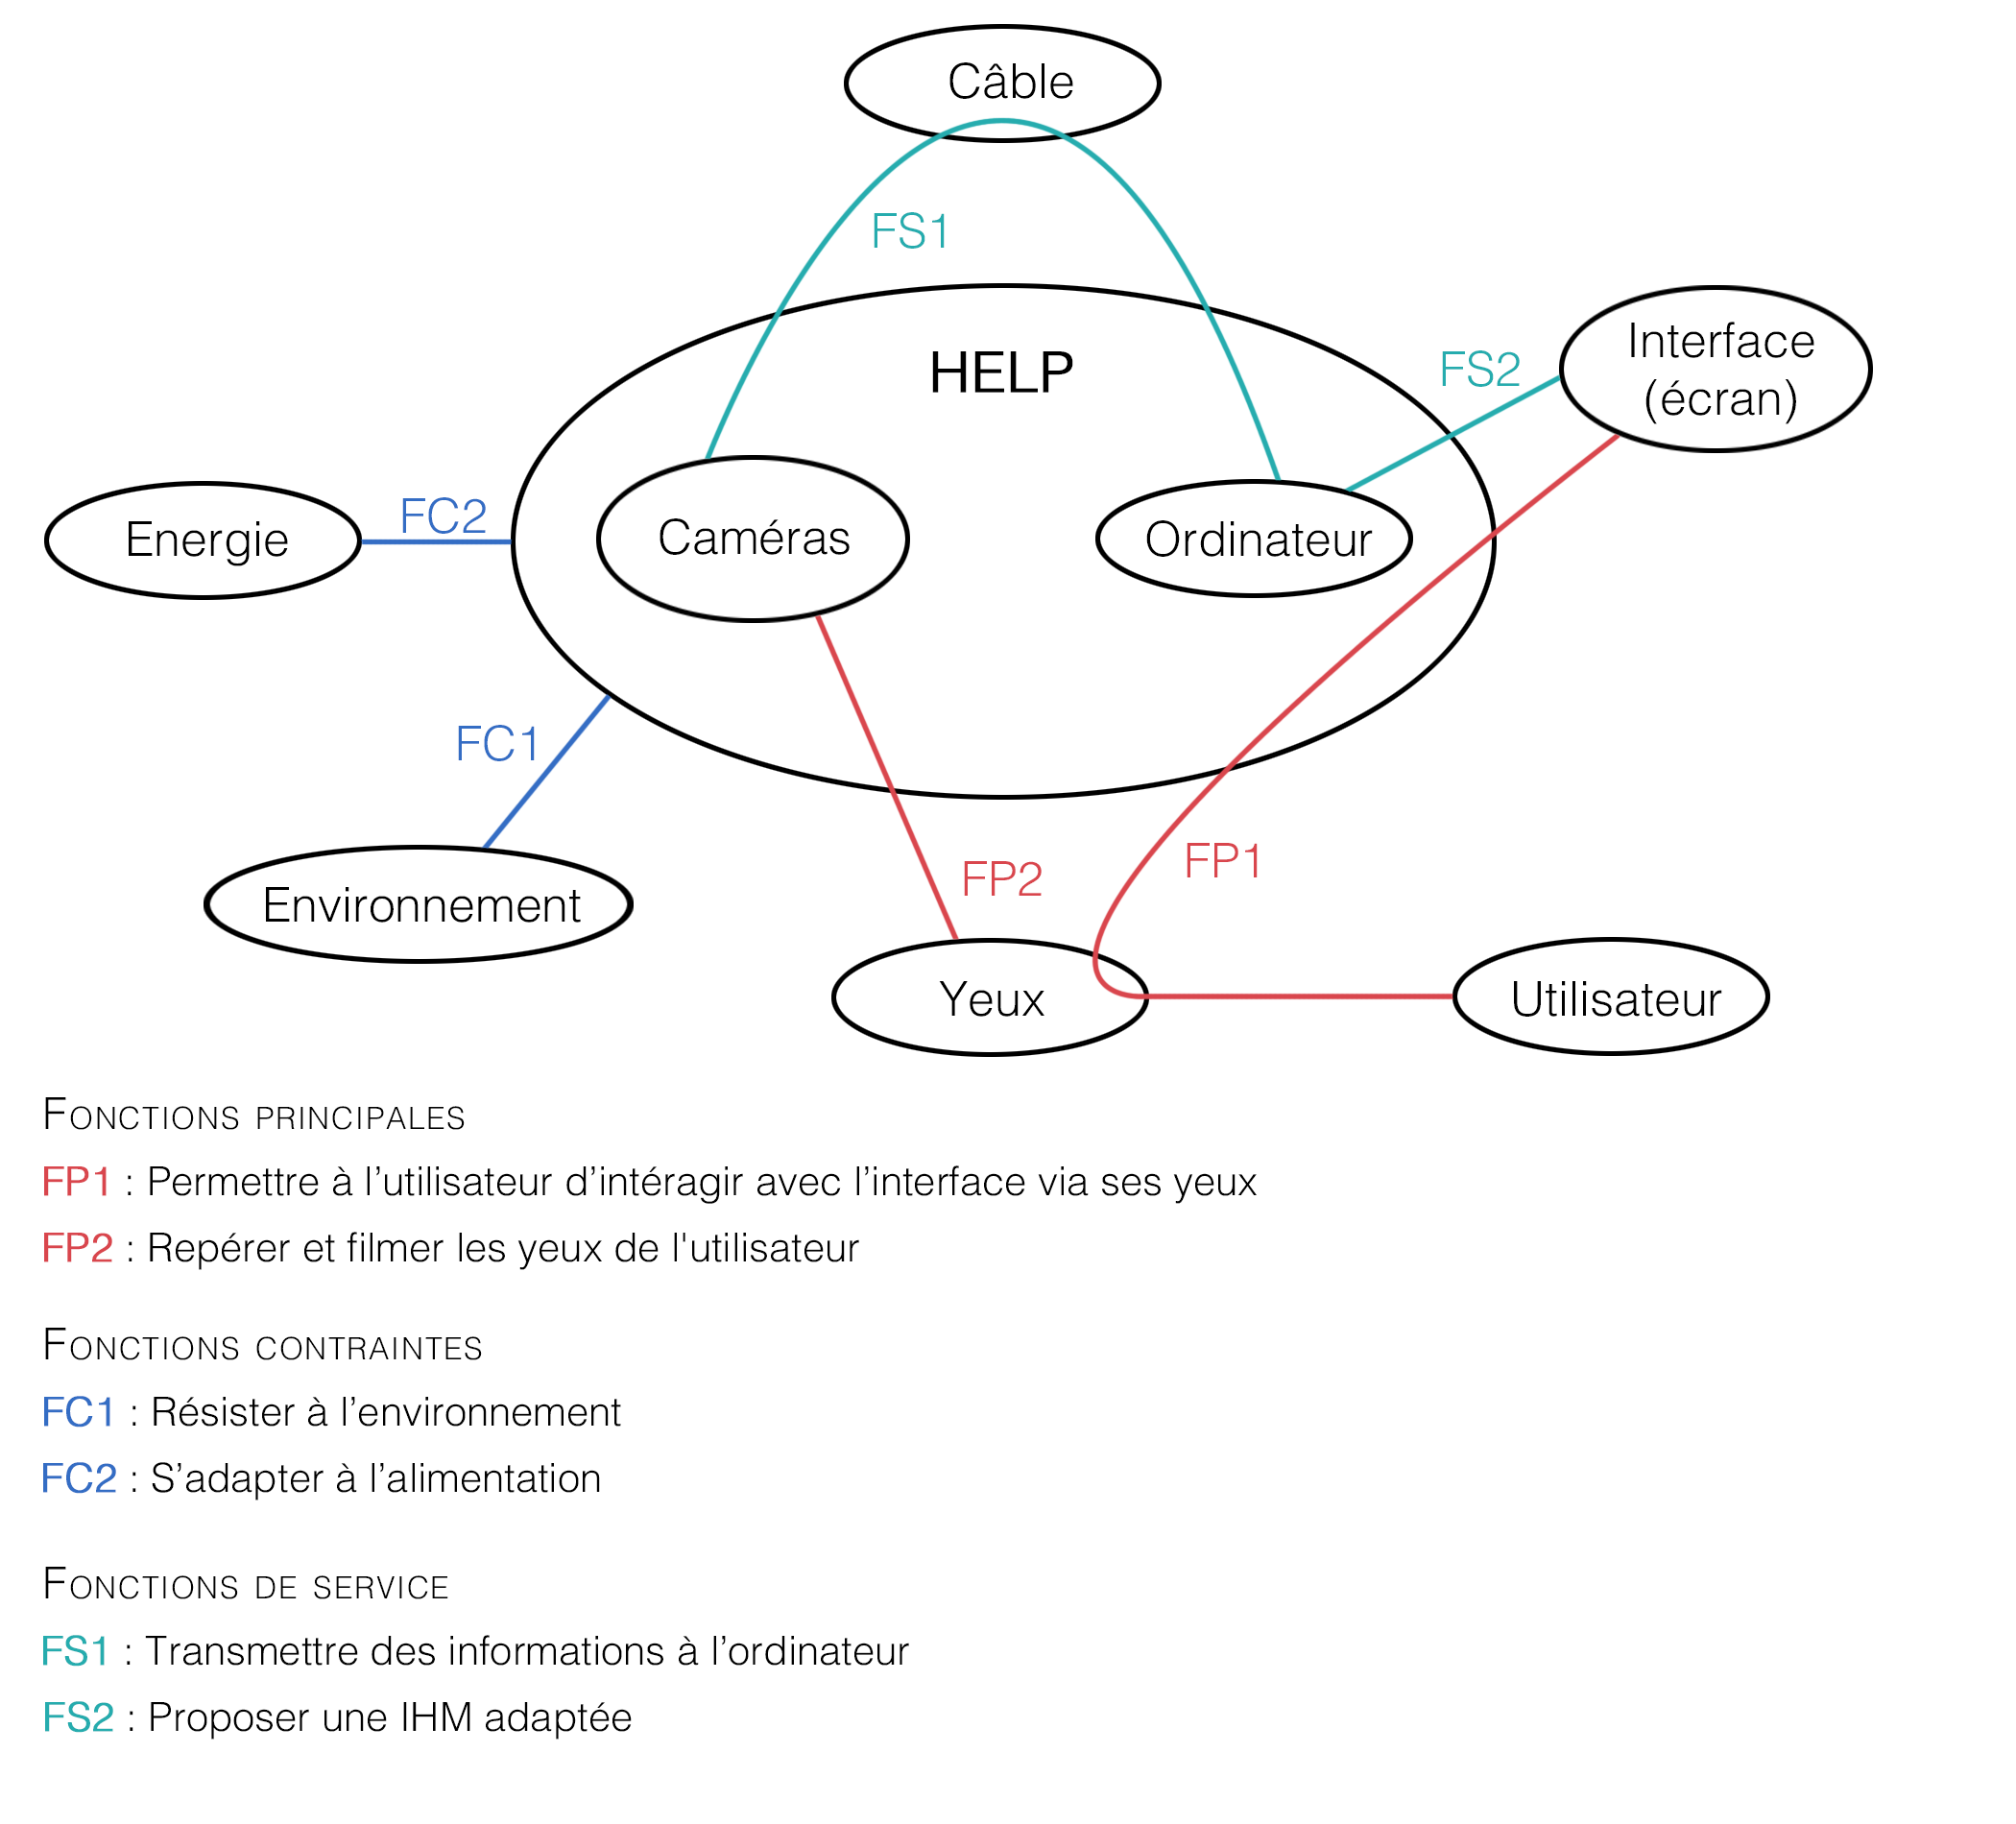
\includegraphics[scale=0.9]{PieuvreV2}
  \caption{Diagramme pieuvre}
  \label{fig:pieuvre}
\end{figure}

\subsection{Approche Bottom-Up}
\definecolor{sable}{RGB}{238,236,225}
Nous avons défini les différentes exigences auxquelles le système devra répondre, indépendamment de nos choix de réalisation technique. Nous les avons alors rassemblées par groupement logique, ce qui nous permettra de définir nos fonctions principales. Les lignes en {\color{sable}{\rule{0.5cm}{0.25cm}}} sont uniquement valables pour la méthode embarquant un système sur l'utilisateur. Elles sont donc à ignorer dans un premier temps puisque nous avons choisi une approche différente. 

\begin{figure}[H]
  \centering
  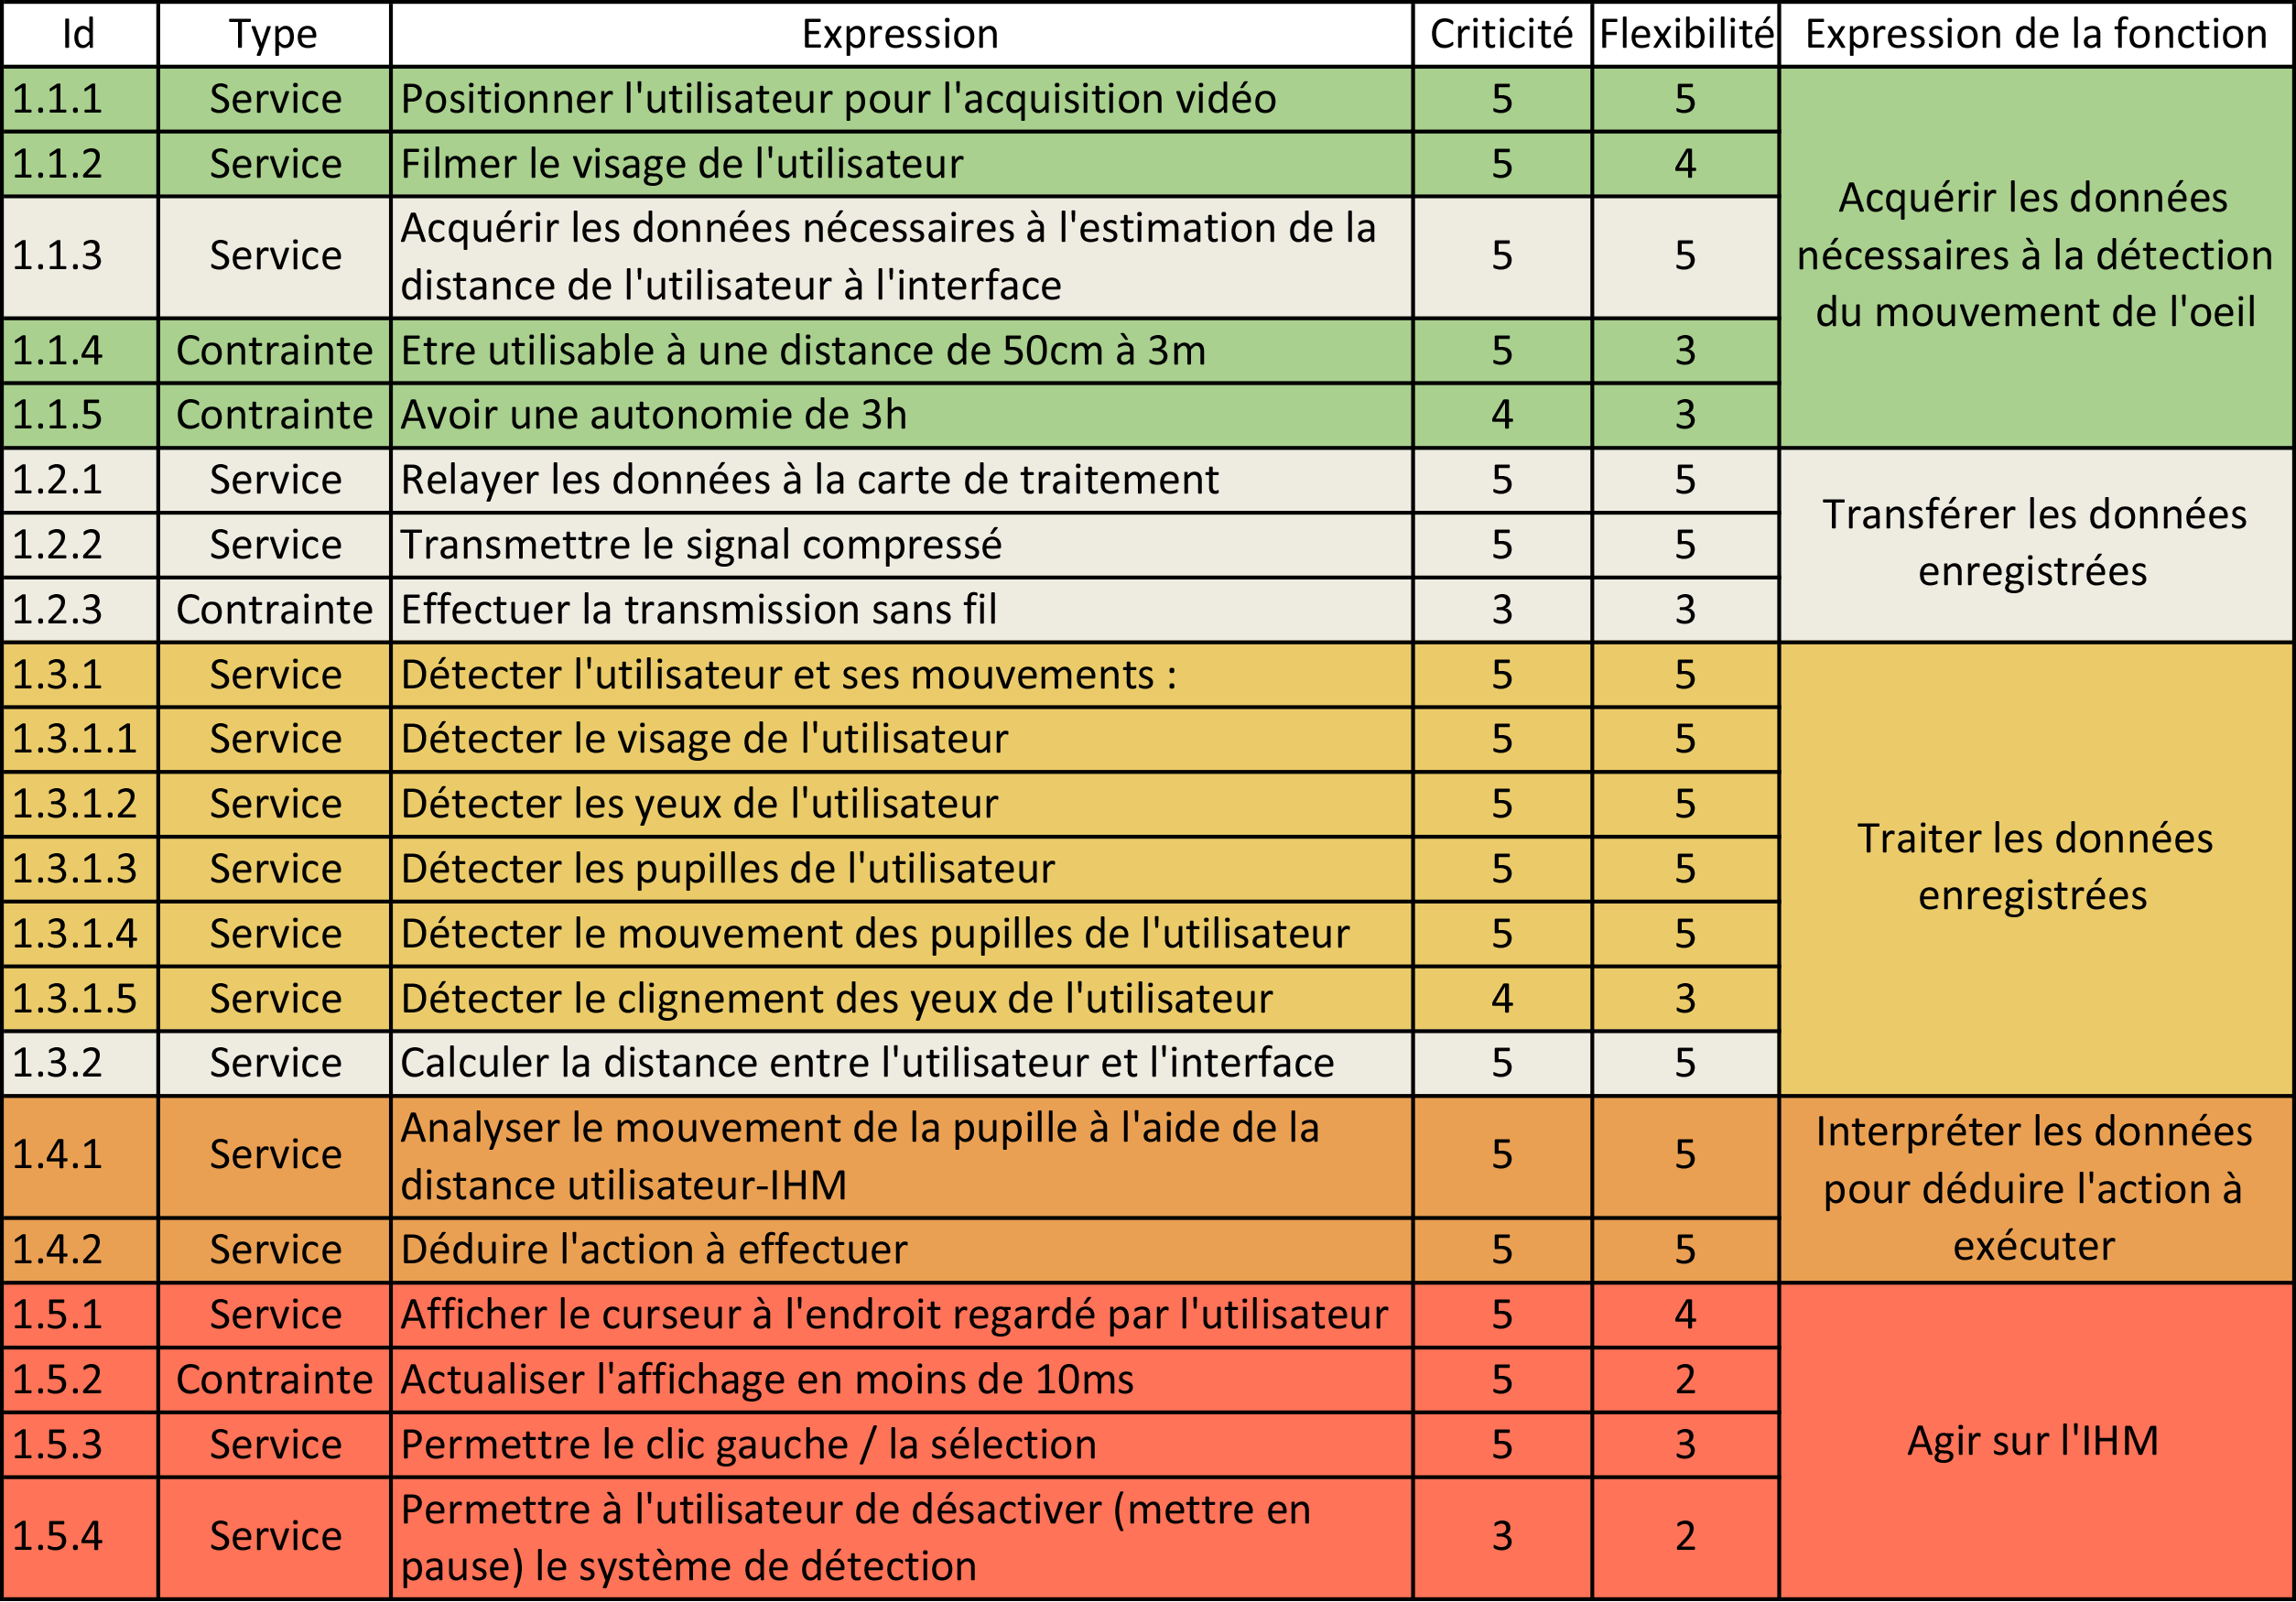
\includegraphics[width=\textwidth]{CahierdesExigencesV3}
  \caption{Cahier des exigences}
  \label{fig:exigences}
\end{figure}

\subsection{Fonctions principales du système}

Dans le cadre de ce projet, nous cherchons donc à remplacer la souris d'un ordinateur par un système qui suit le mouvement des yeux de l'utilisateur. Pour ce faire, nous avons mis en évidence des groupements logiques d'exigence. Tout d'abord, le système doit acquérir les données nécessaires à la détection du mouvement de l'œil. Ces données devront alors être traitées par l'ordinateur. Ce dernier doit alors interpréter ces données pour en déduire l'action à exécuter. De ces nouvelles informations, l'ordinateur doit pouvoir effectuer l'action que l'utilisateur veut effectuer sur l'IHM, la mettre en place, et montrer que ces modifications ont été exécutées. 

\begin{itemize}[label=\textbullet,font=\color{black}]
\item FP1 : Acquérir les données nécessaire à la détection du mouvement de l'œil 
\item\colorbox{sable}{FP2 : Transférer les données enregistrées}
\item FP3 : Extraire les repères anatomiques
\item FP4 : Interpréter les données pour déduire l'action à exécuter 
\item FP5 : Agir sur l'IHM 
\end{itemize}

\section{Spécification fonctionnelle  3 axes}

\subsection{Raffinement FAST}

\begin{figure}[H]
  \centering
  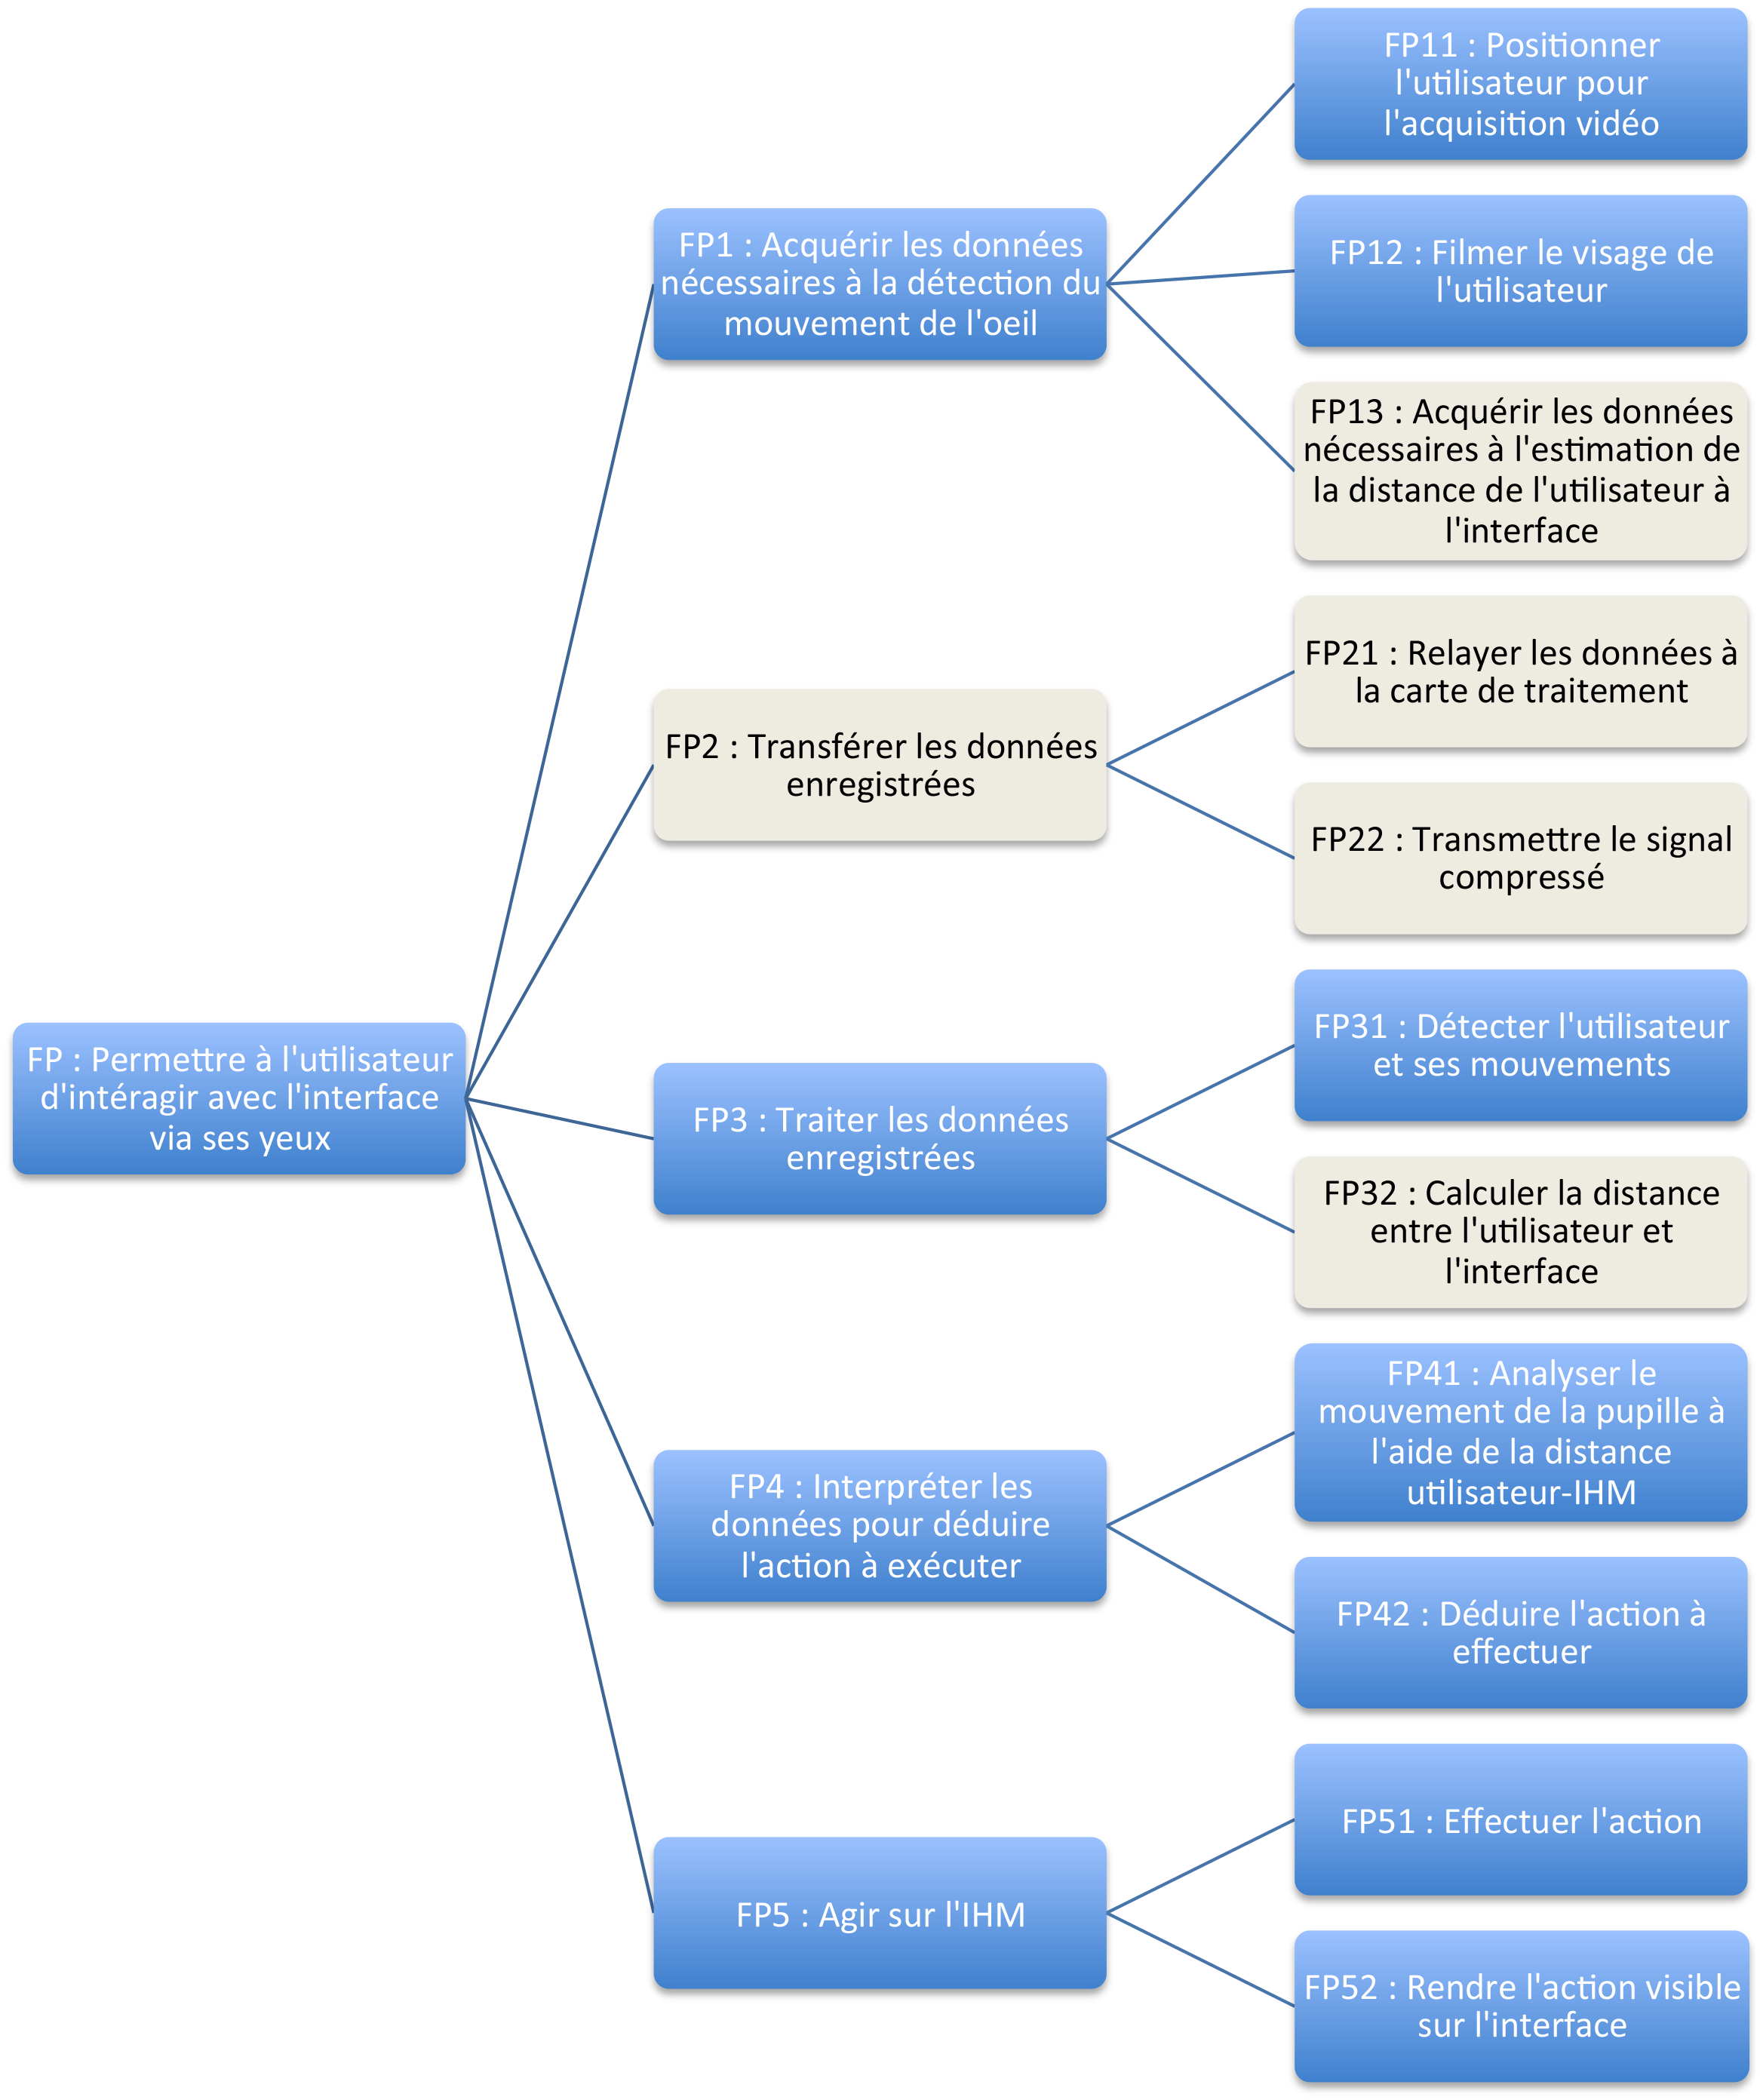
\includegraphics[scale=0.70]{FASTV2}
  \caption{FAST raffiné}
  \label{fig:FAST}
\end{figure}

Le cahier des exigences précédant nous a permis de définir les fonctions principales du système. Nous avons alors cherché à les raffiner par la méthode FAST (cf. figure \ref{fig:FAST}) pour obtenir des fonctions plus précises auxquelles nous pourront apporter des solutions techniques propres à chacune. Nous pouvons ainsi entrevoir l'architecture fonctionnelle.

\subsection{Spécification des données}

La spécification du flux de données va permettre de comprendre les interactions et les échanges entre les différentes parties de notre système. Spécifier ainsi les données nous a permis de mieux comprendre les interactions entre chaque sous-partie du système. Il est ainsi clair que les données que nous allons principalement traiter et transférer seront des flux vidéos et qu’il sera donc important d’optimiser au mieux la rapidité de ces échanges.
Au travers de la figure \ref{fig:fluxDonnees}, nous pouvons aussi voir l’ordre avec lequel les sous-systèmes vont rentrer en jeu. Ainsi la Camera Narrow View sera dépendante du flux envoyé par la Camera Wide View. Un parallélisme de traitement des données est tout de même envisageable sur l'ordinateur pour gérer le flux vidéo de deux caméras.

\begin{figure}[h]
  \centering
  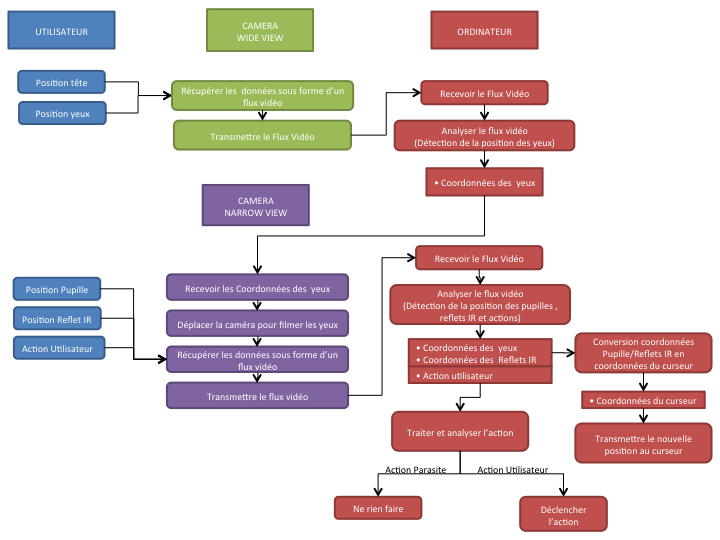
\includegraphics[scale=0.6]{FluxDonnees}
  \caption{Flux de données}
  \label{fig:fluxDonnees}
\end{figure}

\subsection{Spécification des comportements}

Le diagramme de séquence de la figure \ref{fig:comportementGlobal} illustre le comportement global du système. 

\begin{figure}[H]
  \centering
  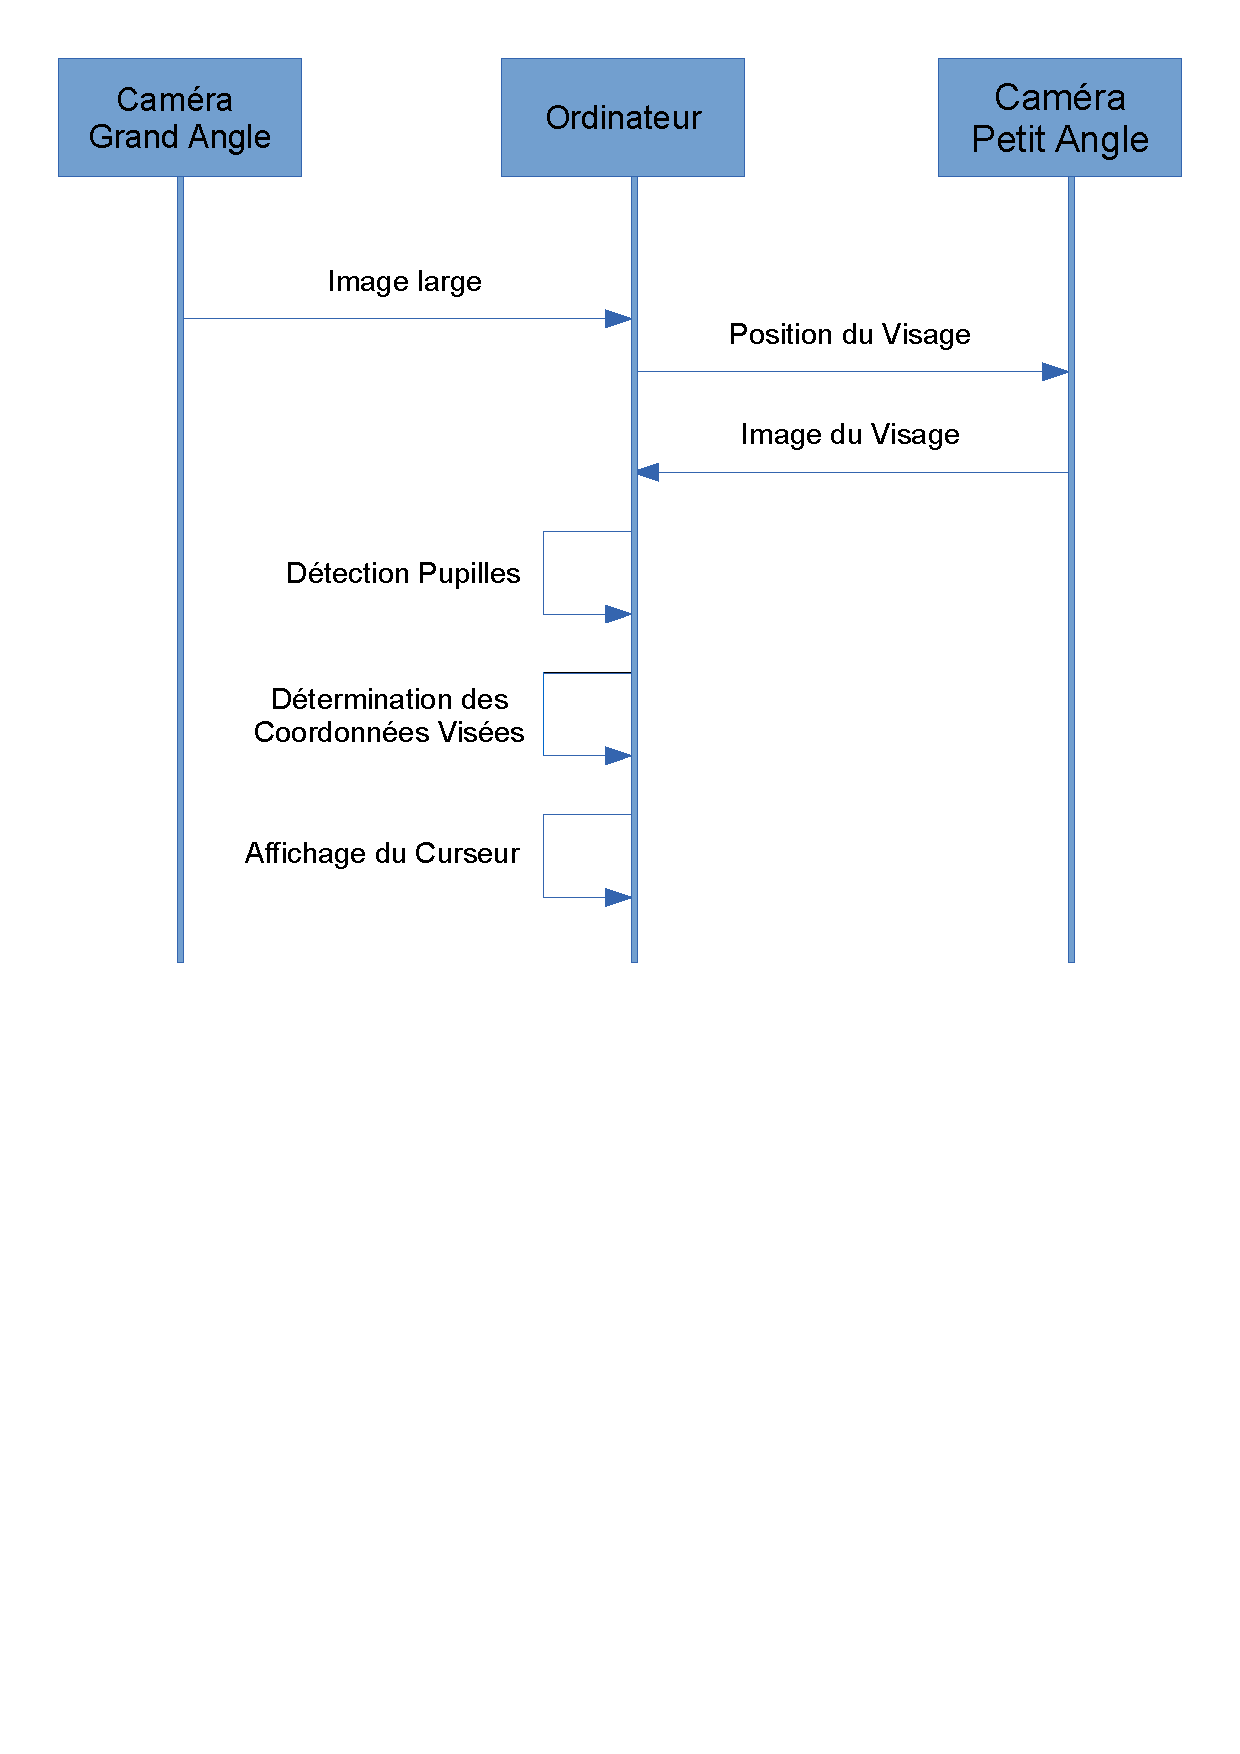
\includegraphics[scale=0.6]{comportementGlobal}
  \caption{Diagramme des spécifications du comportement global}
  \label{fig:comportementGlobal}
\end{figure}

\section{Architecture fonctionnelle}

Tout le travail réalisé au préalable sur la spécification fonctionnelle 3 axes permet finalement de proposer une architecture fonctionnelle pour notre système (cf. figure \ref{fig:archiFonctionnelle}).
 
\begin{figure}[h]
  \centering
  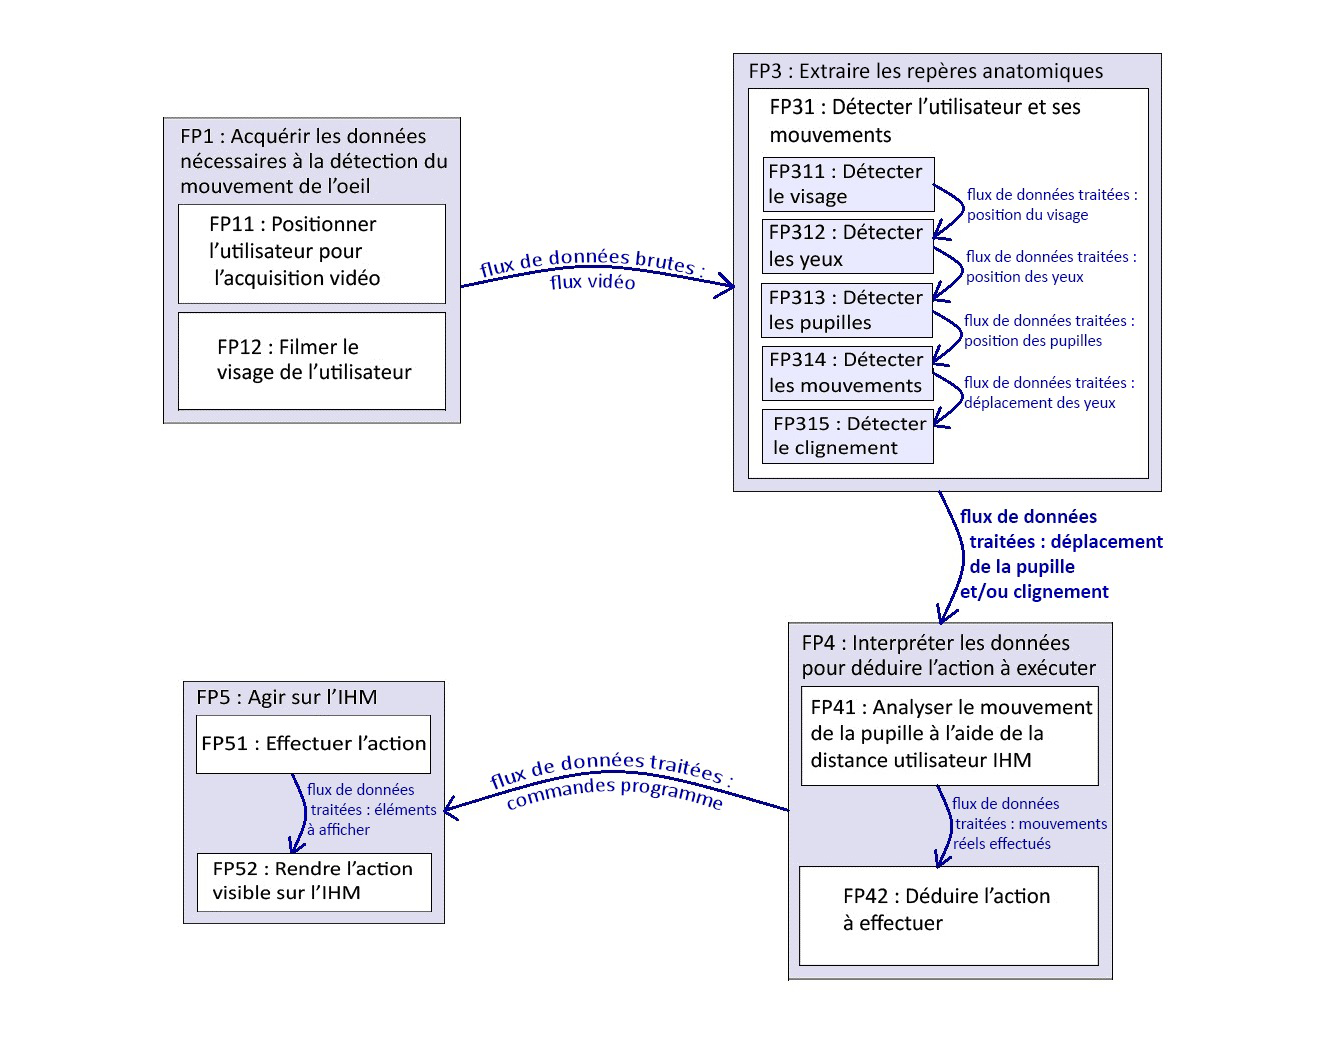
\includegraphics[scale=1.2]{ArchitectureFonctionnelle}
  \caption{Architecture Fonctionnelle}
  \label{fig:archiFonctionnelle}
\end{figure}



%----------------------------------------------------------------------------------------
%	PART III 
%----------------------------------------------------------------------------------------
%\part{Implémentation}
%\chapter{Implémentation}

\section{Architecture physique et interfaces}

Grâce à l'architecture physique (cf figure \ref{fig:archiPhysique}), nous avons pu déduire que notre projet se décomposait en trois sous-systèmes : les interfaces d'acquisition, logicielle et graphique.

\begin{figure}[H]
  \centering
  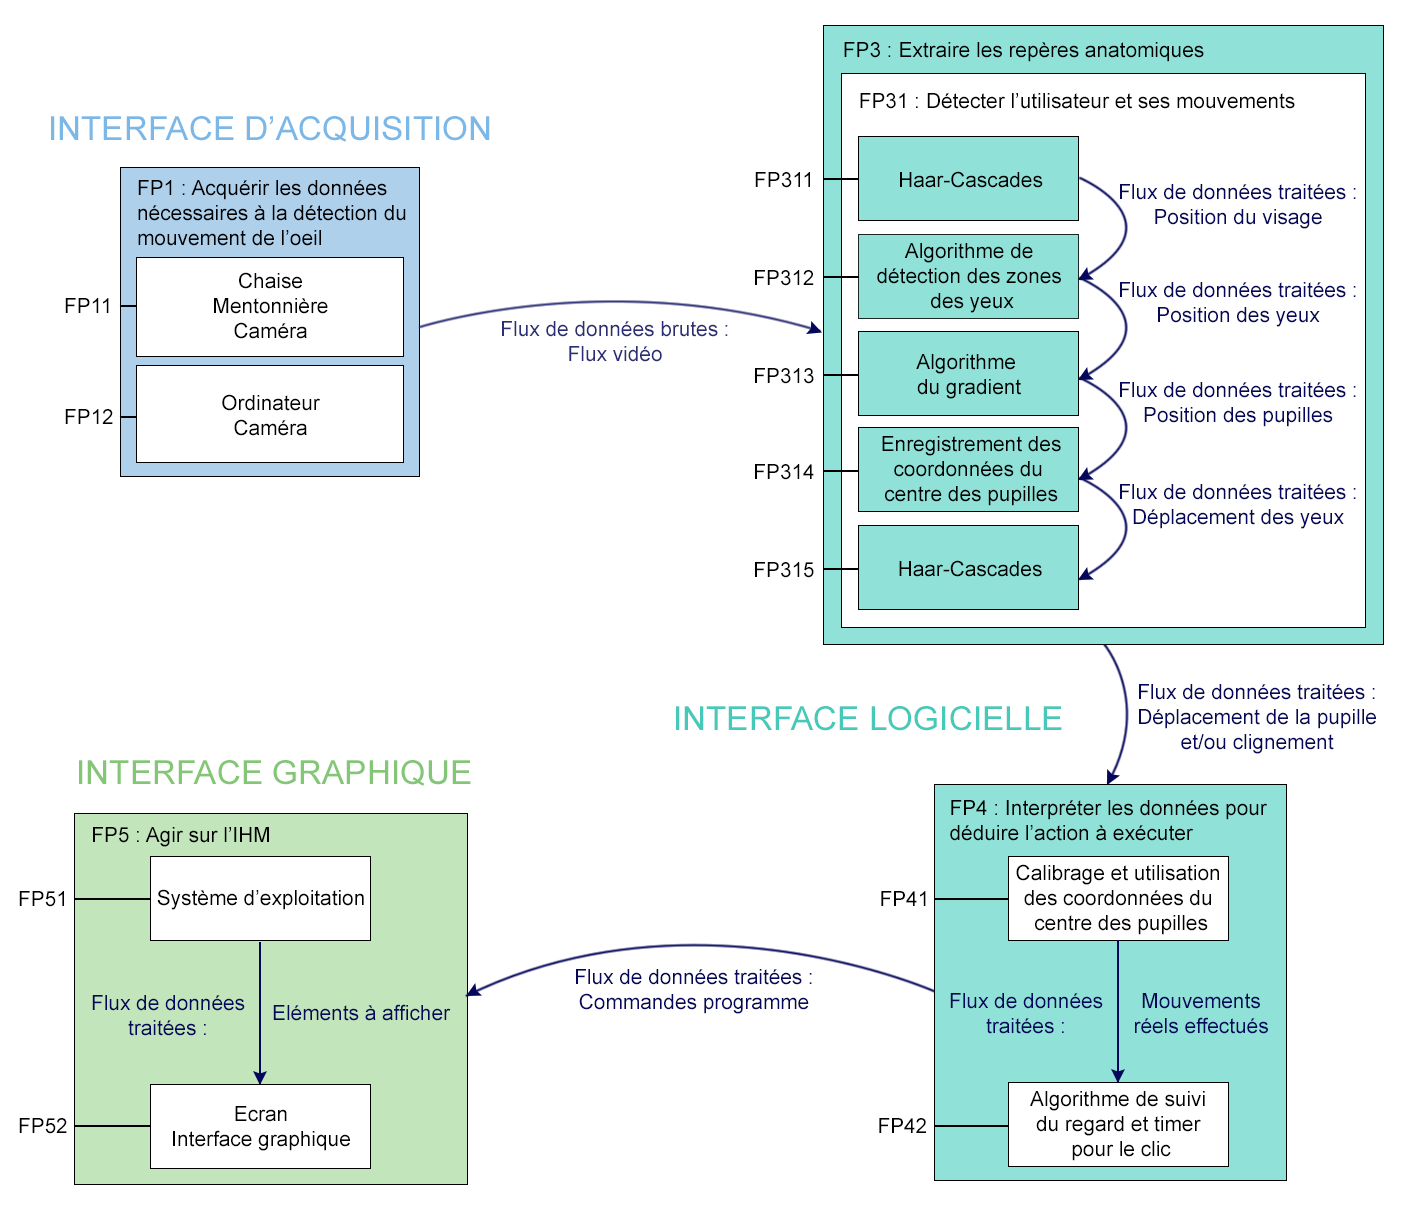
\includegraphics[scale=1.2]{architecturePhysique}
  \caption{Architecture Physique}
  \label{fig:archiPhysique}
\end{figure}

\subsection{Interface d'acquisition}
Cette interface est constituée principalement de la caméra et de la mentonnière (cf figure \ref{fig:systeme}). Cette dernière est utilisée pour éviter les mouvements de la tête, non traités par le programme. L'ordinateur occupe également une place secondaire, puisqu'il permet de vérifier que l'utilisateur est convenablement installé.

\begin{figure}[H]
  \centering
  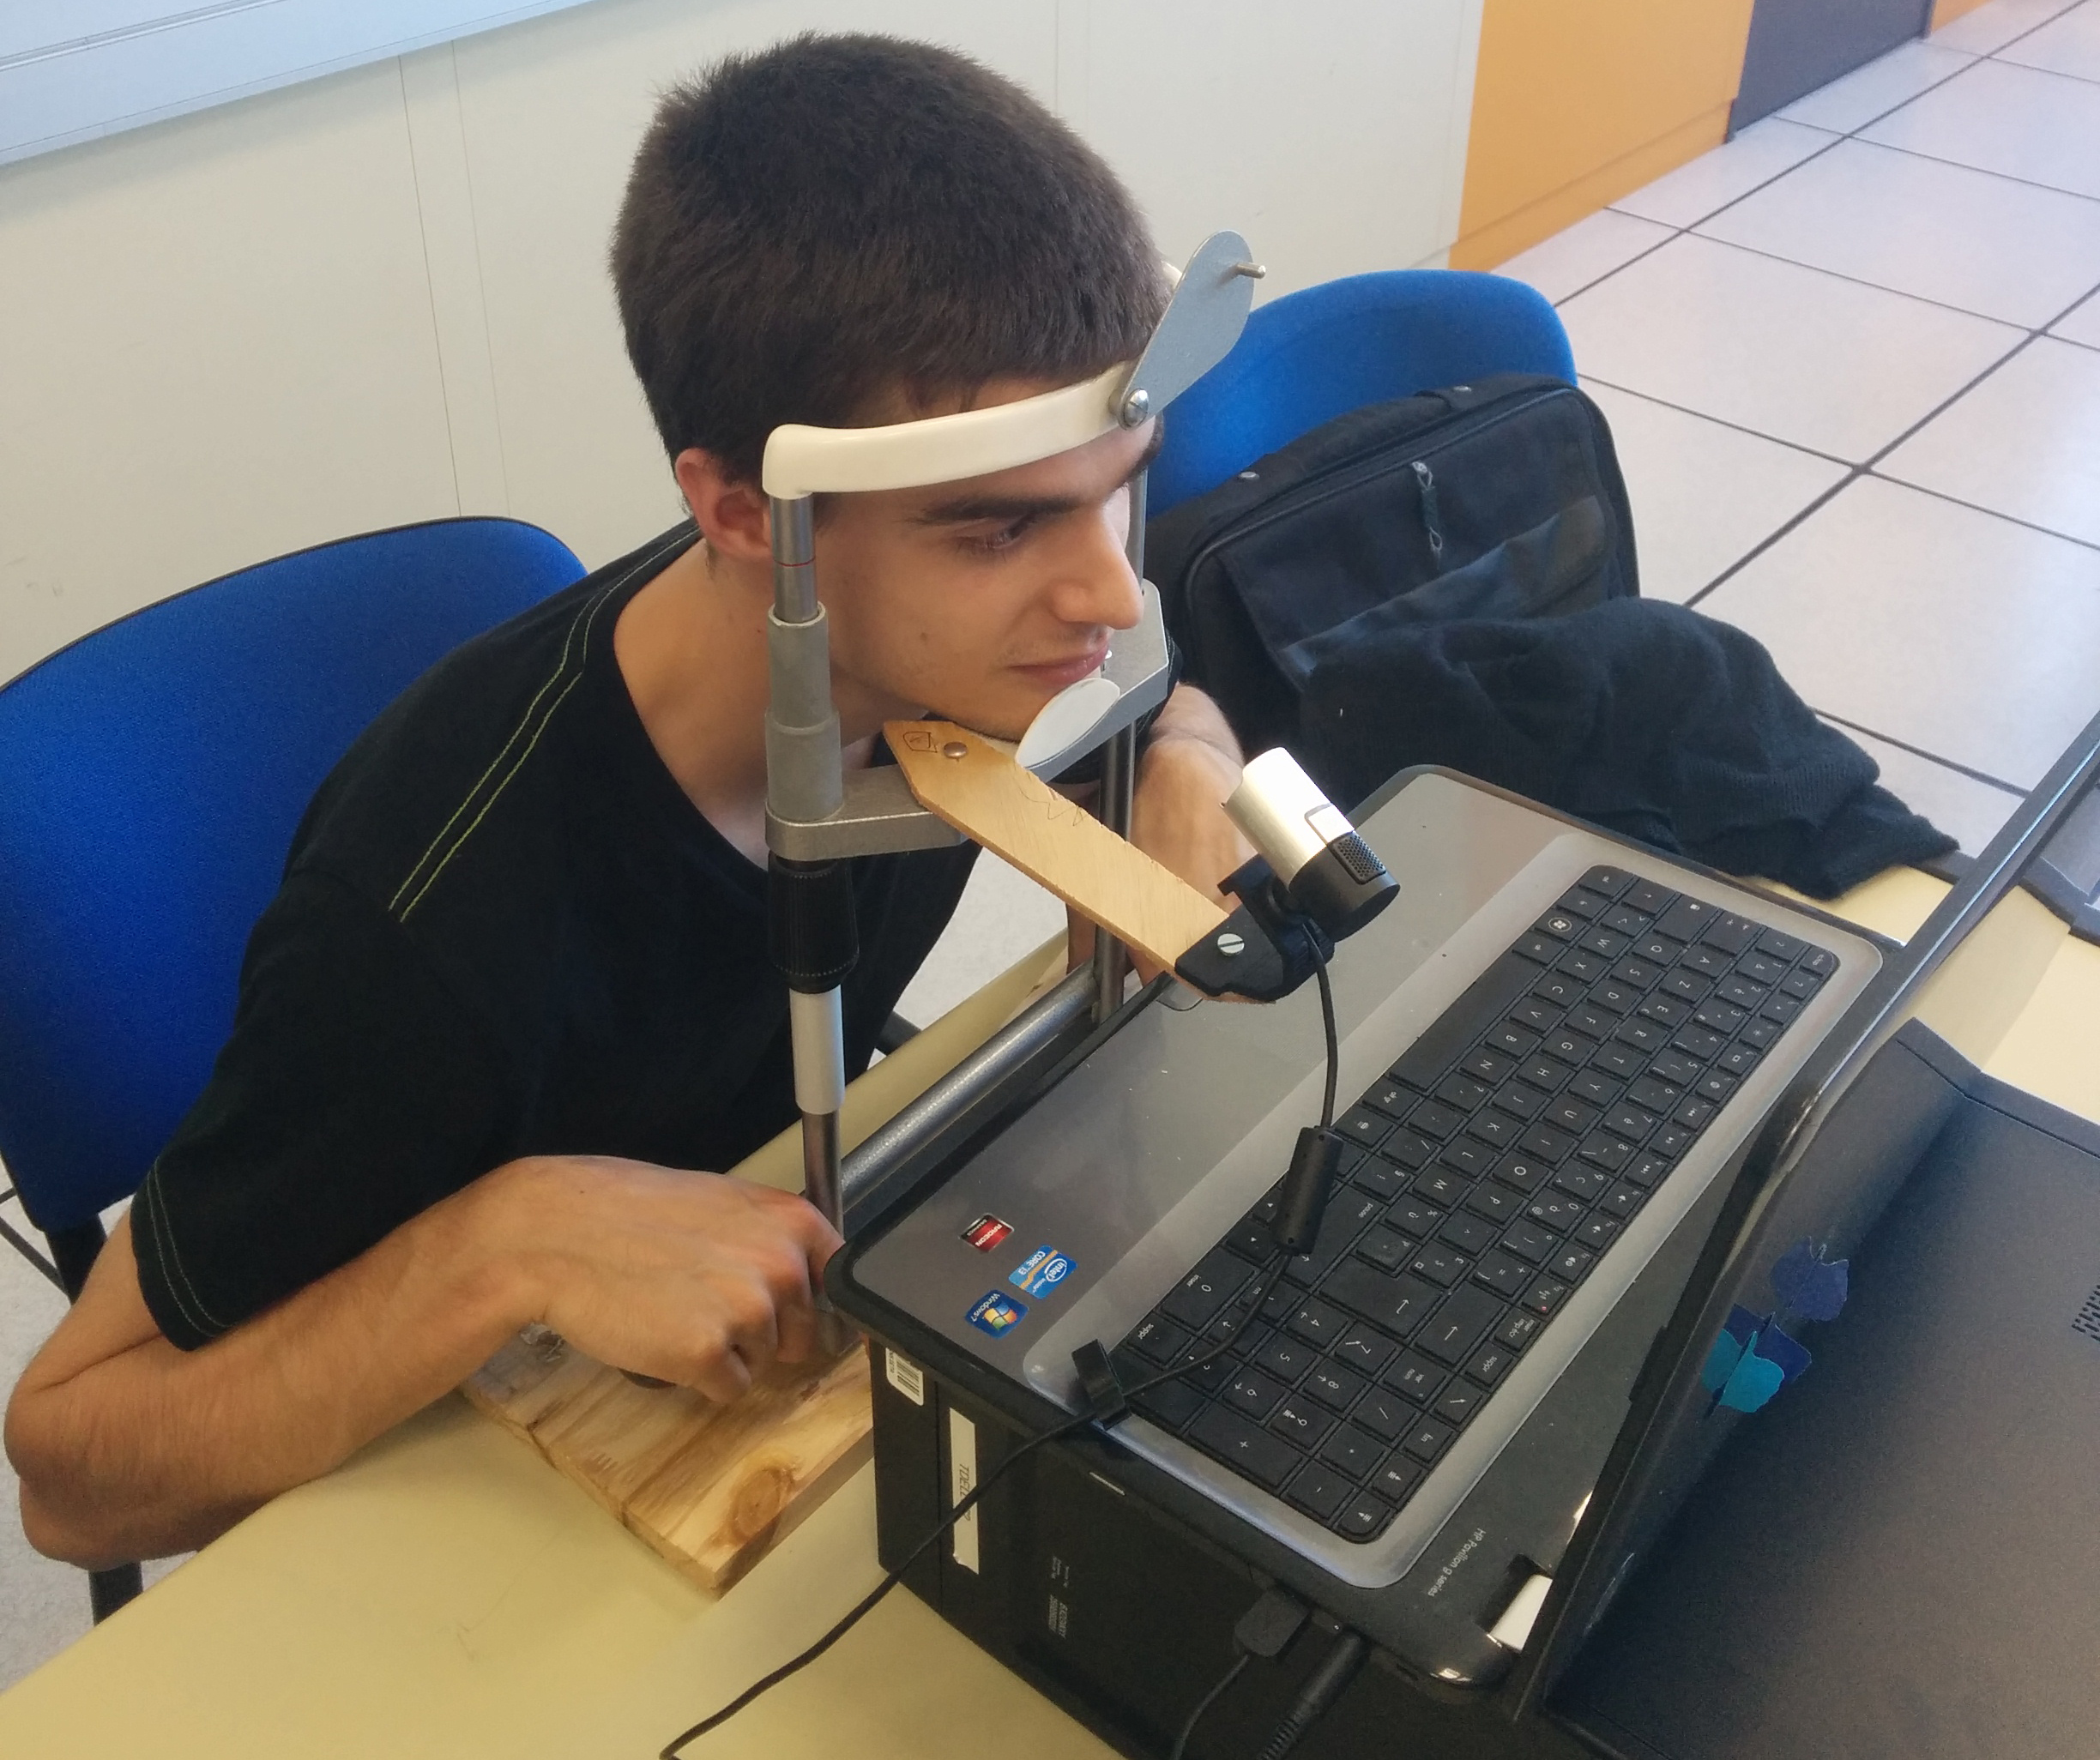
\includegraphics[scale=0.1]{Systeme}
  \caption{Interface d'acquisition composée de la caméra, fixée à la mentonnière}
  \label{fig:systeme}
\end{figure}

\subsection{Interface logicielle}
L'interface logicielle s'appuie sur le programme contenant des algorithmes développés en C++ avec OpenCV. Ils ont pour but de traiter les images transmises par la webcam afin de détecter le visage, puis les yeux et enfin les pupilles et les clignements pour déduire l'action que l'utilisateur souhaite effectuer. Que ce soit pour le clic ou le mouvement du curseur de la souris, une interaction avec l'OS est nécessaire. Le programme doit donc être adapté suivant le système d'exploitation utilisé.

\subsection{Interface graphique}
Enfin, le rôle de l'interface graphique (voir figure \ref{fig:IG9B2}) est de proposer à l'utilisateur un choix de boutons qui lancent des applications. Cette dernière est développée en C++ à l'aide de Qt Creator et ne peut être utilisée que sur Windows car il faudrait changer toutes les commandes d'ouverture d'applications pour exécuter le programme sur un autre système d'exploitation.

\begin{figure}[H]
  \centering
  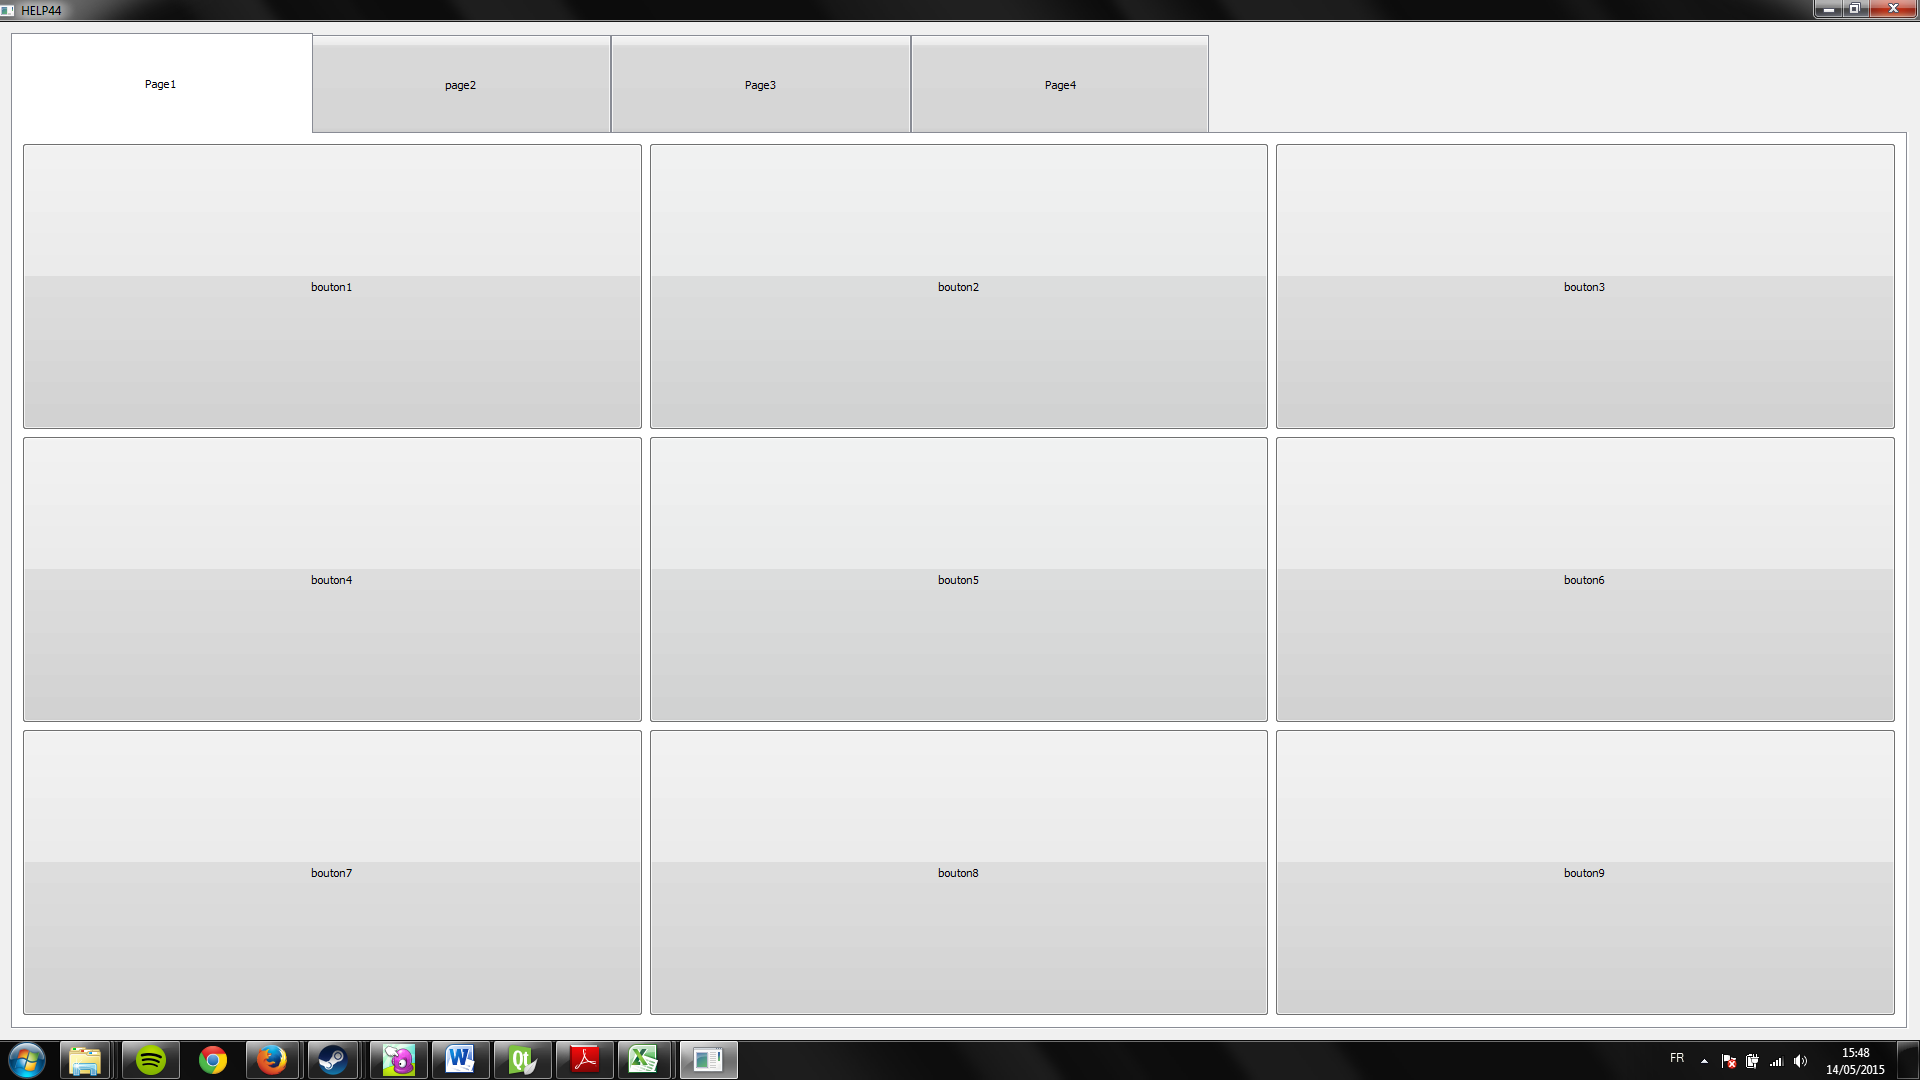
\includegraphics[scale=0.3]{IG9B}
  \caption{Interface graphique 9 boutons}
  \label{fig:IG9B2}
\end{figure}

\section{WBS}
La structure de découpage du projet découle de l'architecture physique. La figure \ref{fig:WBS} illustre le WBS ainsi établi. 

\begin{figure}[H]
  \centering
  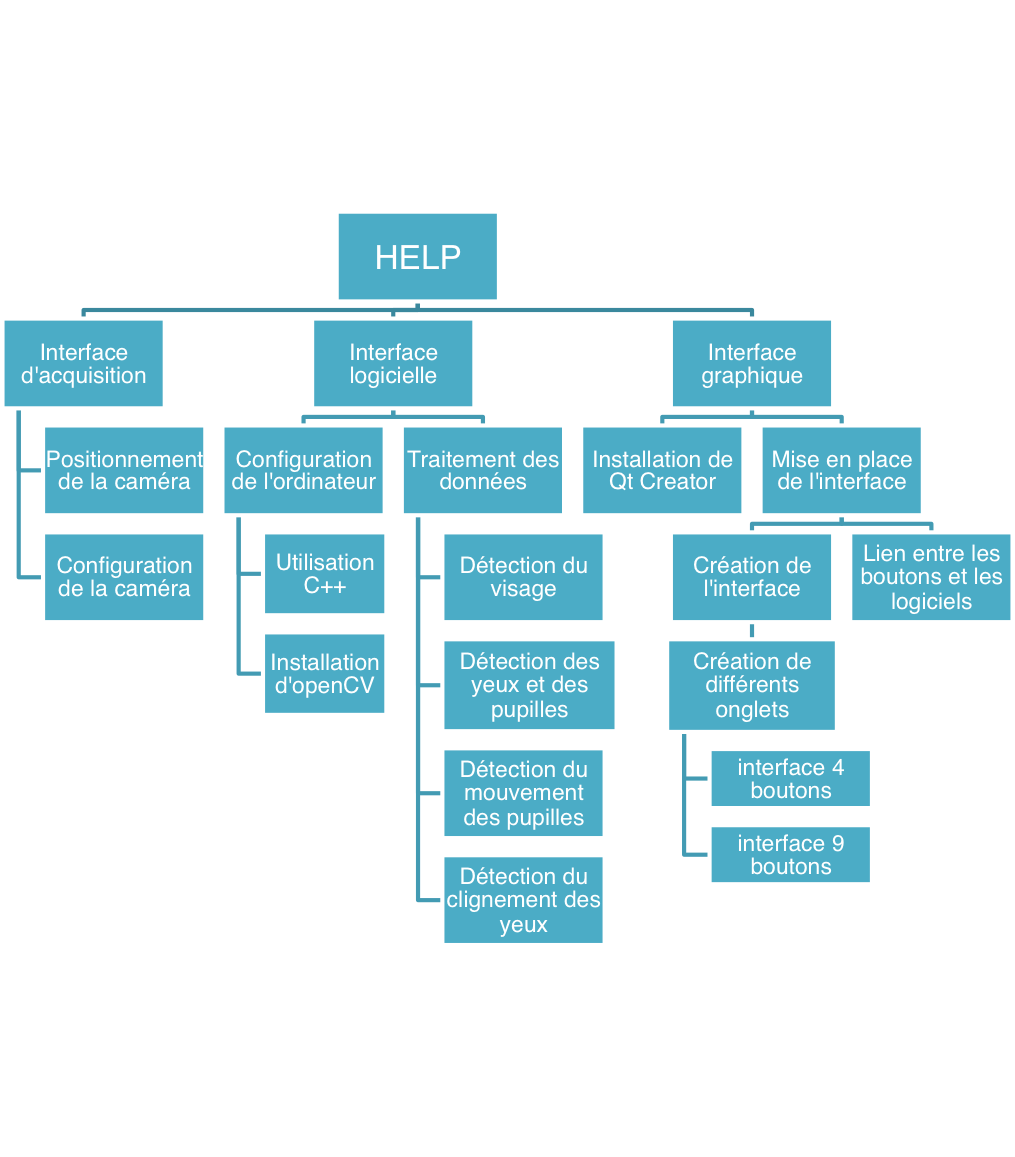
\includegraphics[scale=0.8]{WBS}
  \caption{WBS}
  \label{fig:WBS}
\end{figure}

\section{Matériel utilisé}

Comme présenté sur l'architecture physique, nous avons besoin de matériel pour réaliser notre système.

\subsection{Ordinateur}
L'ordinateur s'est naturellement imposé comme matériel nécessaire au projet, puisque l'utilisateur devait pouvoir utiliser quelques unes de ses fonctionnalités de base. De plus, pour traiter le flux d'images filmées, nous avions besoin d'une puissance de calcul suffisante. Ainsi, l'ordinateur a un double rôle. Il permet d'afficher l'interface graphique, et également d'obtenir l'action demandé par l'utilisateur, grâce à des algorithmes écrits en C++, s'appuiant sur OpenCV. 

\subsection{Caméra}
Si de nombreux types de caméras sont possibles, nous avons retenu la webcam. En effet, la résolution des webcams HD actuelles est largement suffisante pour une détection de pupilles. De plus, elles sont simples d'utilisation, car faciles à installer grâce au port usb d'un ordinateur. Il est aussi aisé de récupérer les flux vidéos. Nous pouvons également noter que les webcams sont relativement peu coûteuses.
Parmi celles-ci, nous avons sélectionné la LifeCam Studio HD 1080p (voir figure \ref{fig:Cam}), pour son bon rapport qualité prix. En effet, la grande résolution HD 1080p (1920x1080) permet un bon tracking des pupilles.

\begin{figure}[H]
  \centering
  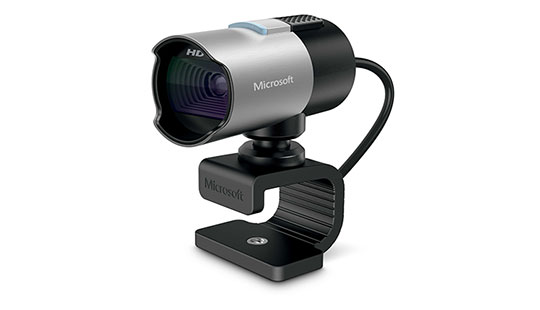
\includegraphics[scale=0.5]{cam}
  \caption{LifeCam Studio HD 1080p \\Source : Microsoft}
  \label{fig:Cam}
\end{figure}

\subsection{Mentonnière}

Afin que les coordonnées du centre des pupilles soient exploitables pour le suivi du regard, nous avions besoin que la tête reste fixe. En effet, lorsque la tête était libre de tout mouvement, les données collectées ne permettait pas de calibrer le programme. La solution de la mentonnière (figure \ref{fig:Menton}) a ainsi émergée. De plus, étant donné que le système vise à être utilisé par la suite par des personnes tétraplégiques, l'immobilisation de la tête ne soulève pas d'incohérence.
Enfin, nous avons fabriqué une planche de bois pour fixer dans un premier temps la caméra près de l'oeil. 

\begin{figure}[H]
  \centering
  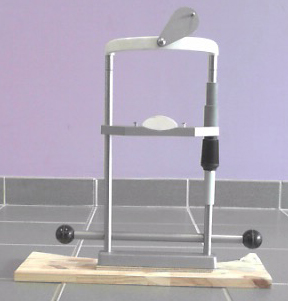
\includegraphics[scale=0.6]{Mentonniere}
  \caption{Mentonnière}
  \label{fig:Menton}
\end{figure}
%\chapter{Interfaces}
%\chapter{Structure de découpage du projet}

SDP en français, ou WBS Work Breakdown Structure en anglais 
%\chapter{Tests unitaires}

%----------------------------------------------------------------------------------------
%	PART IV 
%----------------------------------------------------------------------------------------
%\part{Intégration et validation}
%\chapter{Intégration}

%\chapter{Validation}

%----------------------------------------------------------------------------------------
%	PART V 
%----------------------------------------------------------------------------------------
\part{Organisation}

\chapter{Méthodes de travail}

Méthodes de travail
Organisation temporelle, spatiale, humaine 
interactions des membres de l’équipe projet
interactions avec les encadrants
interactions avec les tiers

\chapter{Outils pour les échanges}

Quels sont les outils qui nous permettent de  travailler ensemble ?

\chapter{Répartition des tâches dans le temps}


WBS et diagramme de Gantt


%----------------------------------------------------------------------------------------
%	PART VI 
%----------------------------------------------------------------------------------------
\part{Journal du projet}
\chapter{Choix et justifications}

\section{Émetteurs infrarouges}

Concernant les émetteurs infrarouges, des LEDs pourront être utilisées. En effet, la distance écran/utilisateur ne sera pas très grande, et de simple LEDs seront suffisantes pour éclairer la pupille de l'utilisateur. Nous pourrons par exemple nous servir de l’Émetteur infrarouge (IR) Kingbright L-934SF4BT (880 nm 50 ° 3 mm) ou alors de l’Émetteur infrarouge (IR) Harvatek HT-159IRAJ 940 nm 20 ° 1206 CMS coûtant respectivement 0.90€ et 0.35€ pièce. Le choix se fera en fonction des connectiques nécessaires (la première LED offre une sortie radiale avec des connecteurs UY2, alors que la seconde se présente sous forme de puce).

\section{Caméras}

Si de nombreux types de caméras sont possibles, nous avons retenu la webcam. En effet, la résolution des webcams HD actuelles est largement suffisante pour une détection de pupilles. De plus, elles sont facilement utilisables via des ordinateurs, c'est-à-dire simple d'installation et il est aisé de récupérer les flux vidéos. Leur connexion USB facilite elle aussi leur emploi. Nous pouvons également noter que les webcams sont relativement peu coûteuses.


\subsection{Caméras «grand-angle»}

Pour le suivi du visage, la Webcam LOGILINK USB avec LED a été retenue. Elle est compatible avec Windows, Mac et Ubuntu et ne posera donc pas de problème de compatibilité. De plus elle possède un système lui laissant la possibilité de pivoter sur 360° permettant ainsi le meilleur suivi du visage possible. Cependant, d'autres webcams présentent ces avantages et le détail qui nous a décidés dans ce choix est la présence de LEDs (voir figure \ref{fig:LEDCam}). En effet, trois LEDs sont présentes de chaque coté de l'objectif et pourraient éventuellement être remplacées par des émetteurs infrarouges.

\begin{figure}[H]
  \centering
  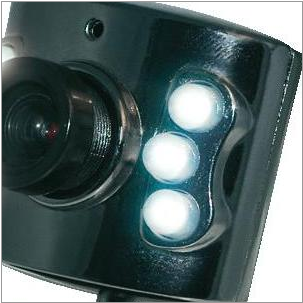
\includegraphics[scale=0.5]{LEDCam}
  \caption{Présence de LEDs sur la webcam}
  \label{fig:LEDCam}
\end{figure}

Le placement des LEDs sur la webcam pourrait nous éviter de devoir mettre en place un système pour pouvoir brancher ces LEDs.


\subsection{Caméras «petit-angle»}

Ensuite, concernant la caméra petit-angle, la Webcam Trust Widescrenn Full HD 1080p (voir figure \ref{fig:CamPetitAngle}) a été choisie. D'abord parce que le tacking des pupilles demande une grande résolution et que cette webcam est adaptée à la résolution Full HD 1080p (1920x1080), mais aussi parce qu'elle intègre un éclairage LED permettant, comme précédemment, de placer nos émetteurs infrarouges.

\begin{figure}[H]
  \centering
  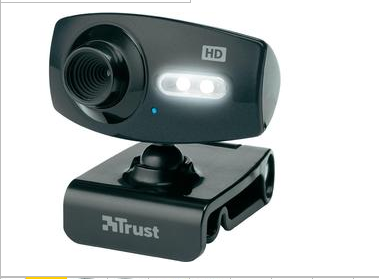
\includegraphics[scale=0.5]{CamPetitAngle}
  \caption{Webcam Trust Widescrenn Full HD 1080p}
  \label{fig:CamPetitAngle}
\end{figure}Émetteur infrarouge

%\chapter{Résultats et analyses}

%analyse des tests et des performances
%analyse des échecs, des décalages et des retards
%Que reste-t-il à faire ? Comment ?






\appendix
\part{Annexes}
\chapter{Première annexe}
\chapter{Deuxième annexe}
\chapter{Troisième annexe}

\backmatter % Partie finale du document, non numérotée

%----------------------------------------------------------------------------------------
%	BIBLIOGRAPHIE
%----------------------------------------------------------------------------------------
\addcontentsline{toc}{part}{Bibliographie}
%\bibliographystyle{apalike-fr}
\bibliographystyle{plain-fr}
\bibliography{bibliographie.bib}
\nocite{*}

%----------------------------------------------------------------------------------------
%	INDEX
%----------------------------------------------------------------------------------------
\cleardoublepage
\phantomsection
\setlength{\columnsep}{0.75cm}
\addcontentsline{toc}{part}{Index}
\label{sec:index}
\printindex

%----------------------------------------------------------------------------------------
%	GLOSSAIRE
%----------------------------------------------------------------------------------------
\cleardoublepage
\phantomsection
\setlength{\columnsep}{0.75cm}
\addcontentsline{toc}{part}{Glossaire}
\printglossaries

%----------------------------------------------------------------------------------------

\end{document}